\chapter{Fragment pose prediction using non-equilibrium candidate Monte Carlo and molecular dynamics simulations} \label{SEH-BLUES}

\small{Authors: Nathan M. Lim*, Meghan Osato, Gregory Warren, David L. Mobley}\\

\section{Abstract}
Part of early stage drug discovery involves determining how molecules may bind to the target protein.
Through understanding where and how your molecules bind, chemists can begin to build ideas on how to design improvements to increase binding affinities.
In this retrospective study, we compare how computational approaches like docking, molecular dynamics (MD) simulations, and a non-equilibrium candidate Monte Carlo (NCMC) based method (NCMC+MD) perform in predicting binding modes for a set of 12 fragment-like molecules which bind to soluble epoxide hydrolase.
We evaluate each method's effectiveness in identifying the dominant binding mode and finding any additional binding modes (if any).
Then, we compare our predicted binding modes to experimentally obtained X-ray crystal structures.
We dock each of the 12 small molecules into the apo-protein crystal structure and then run simulations up to 1 microsecond each.
By studying small and fragment-like molecules, we expect to observe switching of binding modes relatively more quickly than with drug-like or larger molecules.
Following this, we build Markov State Models (MSM) to define our stable ligand binding modes.
We investigate if adequate sampling of ligand binding modes and transitions between them can occur at the microsecond timescale using traditional MD or a hybrid NCMC+MD simulation approach.
Our findings suggest that even with small fragment-like molecules, we do not observe sufficient binding mode sampling and fail to identify all the crystallographic binding modes using microsecond MD simulations, but using NCMC+MD we succeed in sampling all binding modes but do not obtain the correct populations.


\section{Introduction}
High-throughput screening (HTS) is commonly used in early stage drug discovery to identify potential binders or hits.
HTS involves taking a large library of molecules and screening them against a target (e.g. protein)
Hit rates in HTS campaigns are often low, simply due to how vast chemical space can be and the complexity of therapeutic targets \cite{erlanson_introduction_2012}.
One common strategy in fragment-based drug discovery (FBDD) projects is to conduct the screen using smaller molecules (fragments) to cover a larger portion in chemical space which may lead to higher hit rates.
Often in this approach hits tend to be weak binders, but they can serve as a starting point for building a potential lead molecule \cite{erlanson_tethering:_2004}.
From the pool of hits, medicinal chemists may find a desirable starting scaffold or they can build up new molecules by connecting fragments together in hopes to improve binding affinity.
While doing this optimization, chemists must gain an understanding of where and how their molecule binds to their target protein, before they can begin to theorize how to make improvements.

Some experimental approaches to gaining structural insight on ligand binding include X-ray crystallography, nuclear magnetic resonance (NMR), and surface plasmon resonance (SPR).
Each of these approaches present its own set of benefits and challenges but most are costly, time-consuming and difficult \cite{jhoti_fragment-based_2007, gozalbes_contributions_2010}.
For example, X-ray crystallography provides structural information with near atomic-resolution, but obtaining high resolution crystal can be extremely challenging.
Especially with FBDD, resolving the binding mode(s) for small molecules and fragments proves challenging as fragments often bind in several different configurations.
This often produces x-ray structures which have ambiguous densities around the bound ligand or are generally in too low resolution to definitively resolve the fragment binding mode(s) \cite{domagalski_quality_2014}.

Here, with these ambiguous densities in the crystal structures, computational approaches may aid in the design process by resolving ambiguities through predicting fragment binding modes.
Computational methods like docking or molecular dynamics (MD) simulations are some common approaches used in helping to determine fragment binding modes \cite{Rocklin2013BlindSite, durrant_computer-aided_2010, sliwoski_computational_2014}.
If these techniques are accurate enough, computational chemists can apply them to make sense of partial occupancy data and help save structure-based design work which are based on fragments.

Docking is a computationally inexpensive technique which generates a variety of configurations or poses by placing the ligand into a static structure of the apo-protein and subsequently scoring each generated candidate.
It can be performed at high-speeds by neglecting any conformational changes in the protein structures--which often results in sacrificing accuracy--making it difficult to distinguish binders from non-binders \cite{lape_comparison_2010, plewczynski_can_2011, ramirez_is_2018, gohlke_knowledge-based_2000, warren_critical_2006}.
Instead, docking can often be used to understand the conformational space of the ligand and provide some initial insight on how a ligand may fit in the binding site.
Several studies have shown that docking does not reliably find experimental binding modes of ligands \cite{guedes_receptorligand_2013, warren_critical_2006}.
Thus, we use docking to generate a variety of configurations which provide coverage of the entire binding site and use these as starting points for our simulations.

Unlike docking, MD simulations resolve---in full atomistic detail---the overall dynamics of the protein-ligand system by solving Newton's equations of motions in discrete timesteps\cite{hospital_molecular_2015, hollingsworth_molecular_2018}.
This can get very computationally expensive if one wants to simulate biological timescales as MD simulations must take timesteps which are constrained by the fastest motion in the system (i.e. bond vibrations at 1-2 femtoseconds).
One may use schemes like hydrogen mass re-partitioning \cite{hmass_repartition} to enable one to take longer timesteps (i.e. 4fs) by slowing down hydrogen bond stretching, but interesting biological motions occur at much larger timescales necessitating large numbers of timesteps and great computational cost.
Interesting biological motions like protein folding or other large conformational changes have timescales ranges from \(10^{-6}s\) (\(\mu\)s) to \(10^{0}\)s or even longer \cite{han_protein_2014}, requiring extremely long compute times if one aims to capture these types of motions.

Fortunately, recent advancements in technology, like the introduction of computing using graphics processing units (GPUs), have made achieving microsecond (or even millisecond) long MD simulations fairly routine.
Despite using longer timesteps and newer technologies, the utility of MD simulations in the drug discovery process has been hindered by MD's inability to adequately sample the conformational space.
Often, MD simulations of a protein-ligand complex will see the ligand remain trapped in the binding mode the simulation had started in and will fail to capture any transition into alternative binding modes.

For FBDD, MD simulations may hold some value given that fragments are small and rigid enough that transitions between binding modes may occur at shorter timescales.
In this case, MD simulations could then resolve potential binding modes and reveal important stabilizing protein-ligand contacts--that is, if such contacts form on reasonable timescales (nanoseconds to milliseconds).
But in some cases, binding mode transitions may require conformational changes in the protein which may take beyond the millisecond timescale before a transition can even occur \cite{schlick_biomolecular_1997,macek_backbone_2007}.
Although these challenges in adequate sampling of the biologically relevant timescales remain an issue to this day, recent advancements in the field have resulted in new ways to address sampling challenges which we apply within this study.
We note that in this study, we are mostly focused on addressing problems of sampling ligand binding modes that occur in the abscence of slow protein conformational degrees of freedom.

One example of an enhanced sampling approach is a hybrid simulation approach which combines non-equilibrium candidate Monte Carlo (NCMC)\cite{ncmc_paper} move proposals with traditional MD simulations.
We previously implemented this NCMC+MD approach in a software package called BLUES: Binding modes of Ligands Using Enhanced Sampling \cite{BLUES_paper}, which aims to accelerate sampling of ligand binding modes by proposing random rotational moves on the ligand and then runs a conventional MD simulation.
BLUES is similar to using traditional Monte Carlo (MC) moves with MD, except that it uses a gradual non-equilibrium based switching protocol while performing perturbations to the ligand instead of an instantaneous perturbation.
In theory, this allows us to perform larger changes to the ligand, while also increasing acceptance of proposed moves over traditional MC.
With the BLUES approach, we hypothesize that we will observe better sampling of ligand binding modes and be able to identify the experimental ligand binding modes over using traditional MD simulations.
Previous work using BLUES has shown success in accelerating sampling of ligand binding modes in the simple model systems of toluene and iodotoluene bound to the T4 lysozyme L99A mutant \cite{BLUES_paper}.
Here, we are interested in applying BLUES to a more complex target with pharmaceutical relevance to evaluate its utility beyond a simple model system.

In this restrospective study, we are interested in using computational methods to identify binding modes for fragments which bind to a protein called soluble epoxide hydrolase (SEH).
SEH has been hypothesized to have therapeutic potential in cardiovascular diseases, inflammatory diseases, and neurological diseases, which has spurred efforts in developing SEH inhibitors.
Specifically, SEH is involved in the breakdown of epoxyeicosatrienoic acids (EETs), acids with cardiovascular effects such as vasodilation and anti-inflammatory actions.
Through slowing the degradation of EETS (via SEH inhibition), it has been hypothesized to induce neuroprotective, cardioprotective, and anti-inflammatory effects.
In vitro studies with murine models found that SEH inhibition significantly lowered blood pressure, bolstering its hypothesized role in blood pressure regulation \cite{morisseau_impact_2013,morisseau_epoxide_2005,kodani_2014_2015}.

Here, we apply docking, MD, and (NCMC+MD) BLUES simulations on a small set of 12 fragments which bind to SEH and evaluate their effectiveness in identifying their binding modes.
For the remainder of this paper, we define binding modes as experimentally or simulation-determined metastable bound states; ligand poses are defined as the configurations generated from docking.
Prediction of ligand binding modes using MD simulations (in comparison to docking alone) has seen some successes in distinguishing experimental binding modes from decoy poses \cite{liu_exploring_2017,clark_prediction_2016}.
Thus, we will investigate if using microsecond MD simulations or our BLUES  (NCMC+MD) enhanced sampling approach provide any value, beyond docking, for identifying the SEH fragment binding modes.
We will compare poses generated from docking and the metastable binding modes sampled from MD and BLUES against experimentally obtained x-ray crystal structures.
Through this study, we aim to provide insight on the value computational methods can provide in identifying the crystallographic binding modes and finding additional binding modes.

\section{Methods}
\subsection{SEH apo-protein preparation}
Prior to beginning this study, our OpenEye Scientific collaborators provided the SEH structure, the location of the binding site where ligands would be docked, and a set of 47 ligands in the form of SMILES strings.
The initial SEH structure from OpenEye Scientific was missing residues.
We found the apo SEH structure in the Protein Data bank (PDBID:5AHX), built in the missing residues with PDBFixer, and used this structure for the remainder of the study \cite{noauthor_pdbfixer_2019}.
The apo SEH structure was altered using the PDB2PQR web server \cite{pdb2pqr}, which uses PROPKA2.0 to assign residue protonation states.
We protonated residues at pH 8.5 to match experimental conditions, using AMBER parameters \cite{jurrus_improvements_2018,sondergaard_improved_2011,noauthor_propka3:_nodate} and we removed crystallographic waters from the system.
The PQR file was then converted back to a PDB file with ParmEd (v3.0.1).
We aligned the corrected apo SEH structure to the SEH structure provided by OpenEye Scientific to ensure the pre-defined docking site was the same.

\begin{figure}
    \centering
    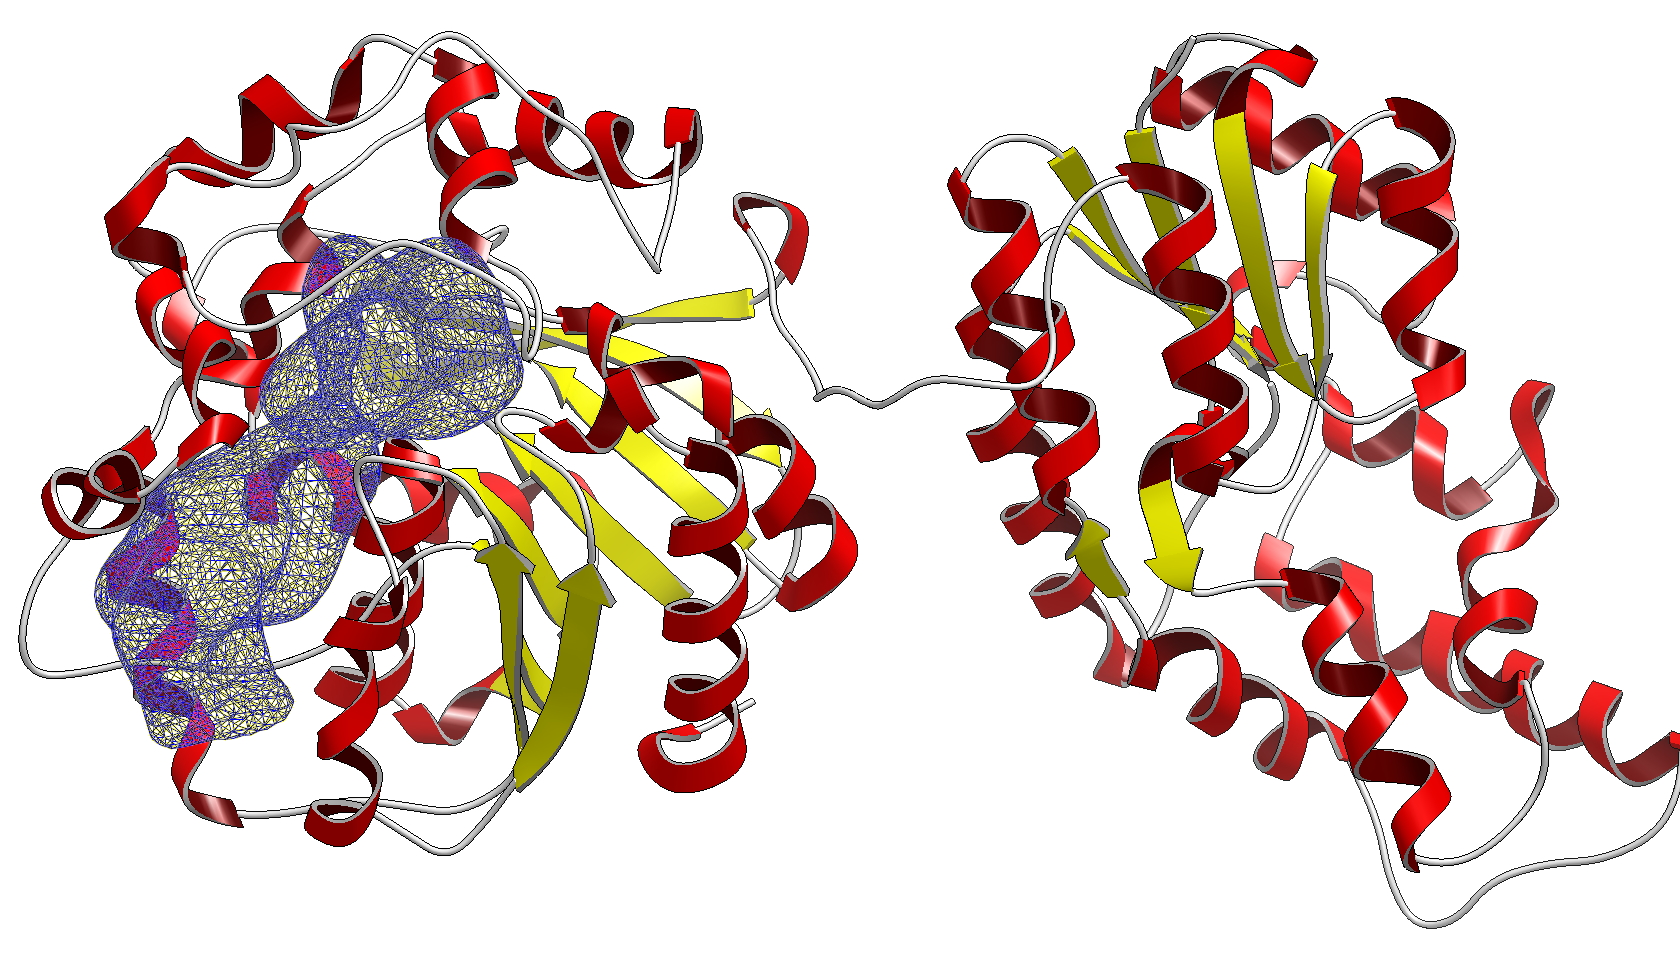
\includegraphics{chapter6/Figures/fullprotein.png}
    \caption[SEH Complete Protein]{The complete SEH protein structure with the C-terminal domain (left) and the N-terminal domain (right). The docking site is highlighted (blue) in a mesh representation. The N-terminal domain (right) was removed to reduce computational costs, keeping the C-terminal domain with the defined docking site.}
    \label{fig:full-protein}
\end{figure}

\begin{figure}
    \centering
    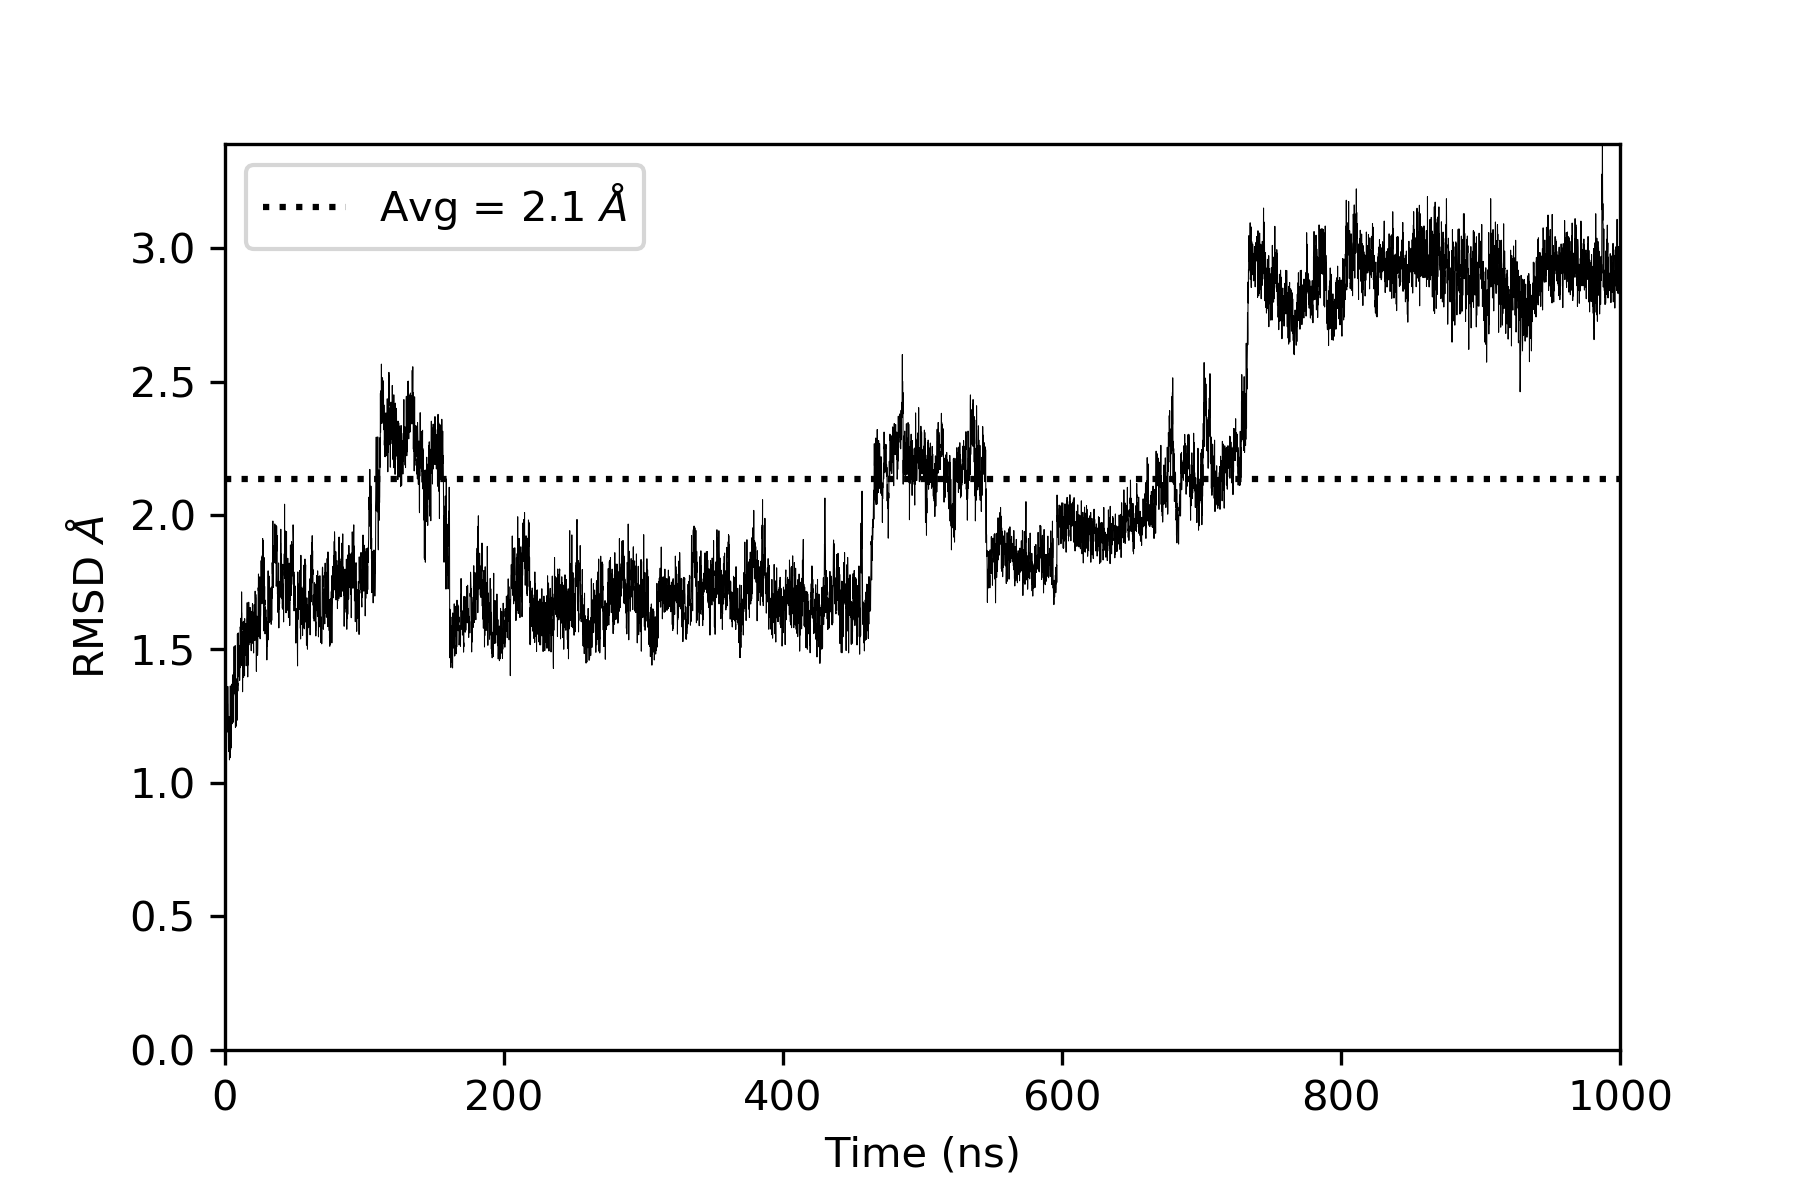
\includegraphics{chapter6/Figures/protein-bb-rmsd.png}
    \caption[SEH Backbone RMSD after N-terminal domain removal]{Calculated RMSD {\AA} of the protein backbone relative to the starting position for 1 microsecond of MD with an average RMSD of 2.1 {\AA} after removal of the N-terminal domain. The protein backbone eventually stabilizes at 3 {\AA} from the starting position. This indicates that removal of the N-terminal domain did not largely affect the protein structure.}
    \label{fig:protein-bb-rmsd}
\end{figure}

The SEH protein contains 2 domains, a phosphatase domain (N-terminus) and a hydrolase domain (C-terminus) connected by a flexible proline rich linker \cite{doi:10.1021/bi050842g}.
The pre-defined docking site was only located in the C-terminal hydrolase domain, so to reduce computational cost, we removed the N-terminal domain from residue 0 to residue 224 (Fig. \ref{fig:full-protein}).
We analyzed the structural integrity of the truncated protein by averaging the RMSD of the protein backbone over a 1 microsecond MD simulation.
The average RMSD of the truncated protein backbone was 2.1 Angstroms suggesting the C-terminus was relatively unaffected by the removal of N-terminus.
In Figure \ref{fig:truncated-protein}, we show the entire binding site located in the C-terminus domain as defined by our collaborators.

\begin{figure}
    \centering
    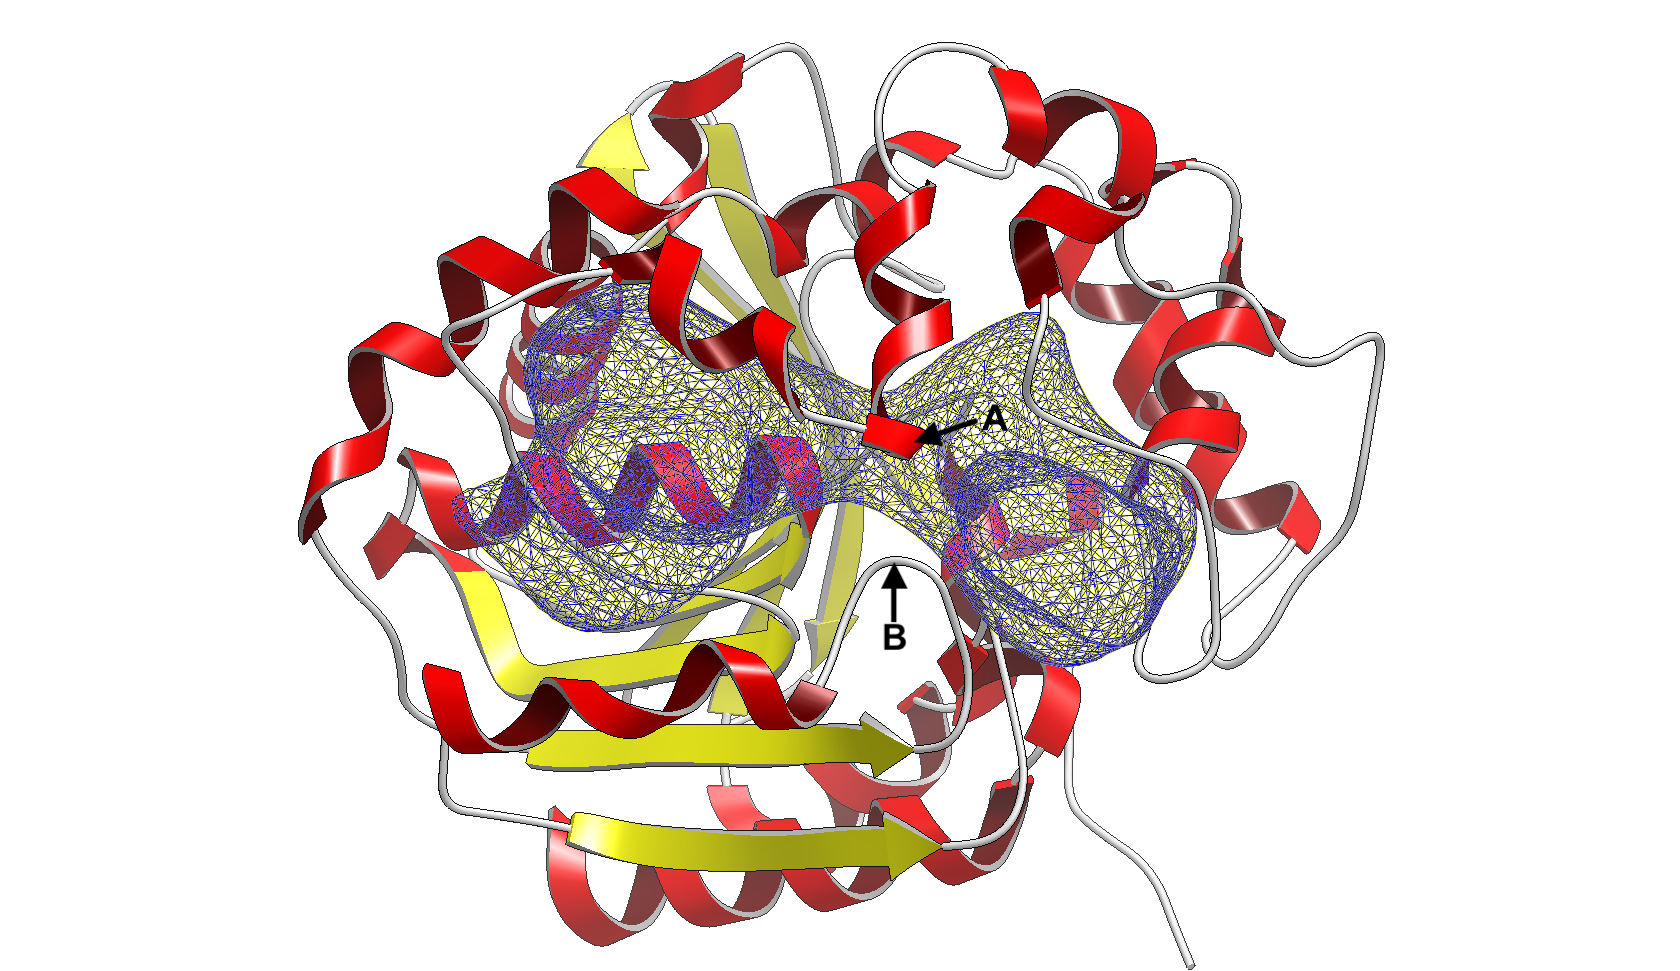
\includegraphics{chapter6/Figures/protein-mark.png}
    \caption[Truncated SEH Protein Structure]{Truncated SEH protein structure (C-domain only) with the the docking site is highlighted (blue) in a mesh representation. We divide the full cavity into two sub-cavities denoted by left and right. The sub-cavity division is best denoted at the two loops marked as A and B in the figure. In the SEH apo protein structure, point A is closest to residue VAL381 and point B is closest to residue VAL499. We treat each sub-cavity separately in our analysis to better resolve binding modes within each sub-cavity.}
    \label{fig:truncated-protein}
\end{figure}

Here, we define two sub-cavities (left/right) which are separated by two loops which form at residues VAL381 (A) and VAL499 (B), creating a cleft in the center of the SEH binding site (Fig. \ref{fig:truncated-protein}).
Throughout this study, we treat the left and right sub-cavity separately as we did not observe transitions between them in our simulations.
By performing our analysis on each sub-cavity separately, we are better able to resolve the binding modes and timescales for transitions between binding modes, over trying to resolve the transition timescales between the sub-cavities.

\subsection{Ligand preparation and docking}
\begin{figure}
    \centering
    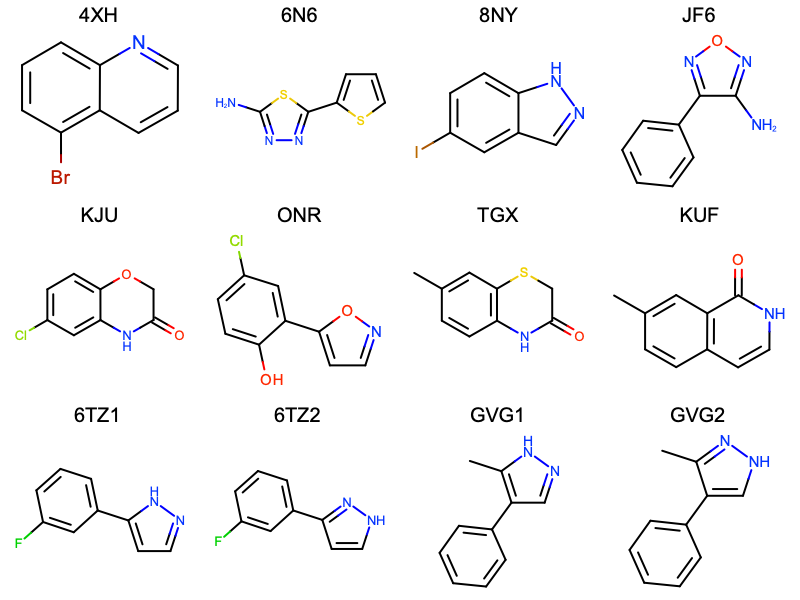
\includegraphics{chapter6/Figures/2dmolecules.png}
    \caption{}
    \label{fig:2dmolecules}
\end{figure}
From a set of 47 ligands given to us by our OpenEye Scientific collaborators, we chose to study a smaller subset of 12 ligands (Fig. \ref{fig:2dmolecules}).
Here, we chose ligands based on the overall size and number of rotatable bonds.
Particularly, we were interested in only studying small and rigid fragment molecules as we expected to observe more binding mode transitions during our simulations, due to their size and rigidity.
The molecule set ranged from 133.13 to 156.73 ${\AA^{3}}$ in shape volume with 0 to 1 rotatable bonds.

We used openmoltools (v0.8.1) \cite{} and OpenEye toolkits \cite{openeye_toolkit} to convert each ligand SMILES string to a 3D structure and then we assigned charges using the OEAM1BCC \cite{jakalian_fast_2002}. charging scheme from the OEQUAPAC library \cite{jakalian_fast_2002}. .
Then, we generated 1000 conformers of each charged ligand using OpenEye’s OMEGA (20180212) \cite{hawkins_conformer_2010}.
These conformers were then docked into the SEH apo protein structure using FRED from OEDock(v3.2.0.2), generating 1000 docked poses, and scored with the Chemgauss4 scoring function \cite{mcgann_fred_2011}.

\begin{figure}
    \centering
    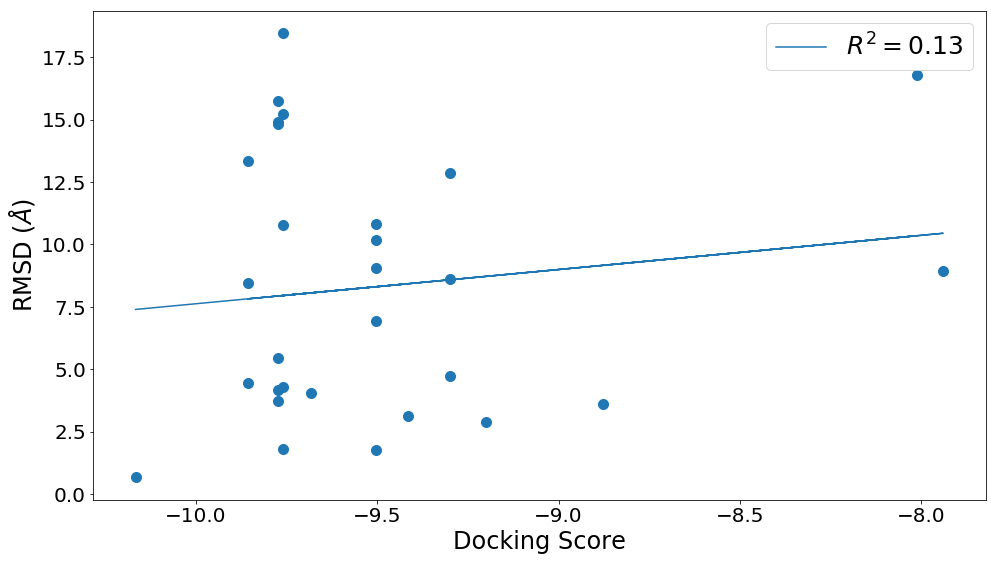
\includegraphics{chapter6/Figures/topscore.png}
    \caption{Docking score and the calcualted RMSD {\AA} to the crystallographic binding modes from the top scoring docked poses.}
    \label{fig:topscore}
\end{figure}

From the 1000 generated docked poses, we wanted to select the most distinct and use them as our starting positions for our simulations.
Here, we define distinct docked poses as poses which are dissimilar from one another.
Some studies have shown that docking is an unreliable method for identifying the true binding mode using the top scoring pose \cite{warren_critical_2006}.
Given this, we believed that the top scoring poses would often be far from the true binding mode and thus, we did not retain them and use them as starting points for our MD simulations.
Later, we confirmed that the top scoring docked poses are not generally close to the crystallographic binding modes (Fig. \ref{fig:topscore}).

By selecting the distinct poses generated from docking, we have a variety of starting configurations in our simulations and provide reasonable coverage of the protein binding site.
Regardless of the starting positions, given enough simulation time and the fragment-like properties (i.e. small and rigid properties) of the molecules we are simulating, we should see convergence to the true binding mode given the forcefields, protonation states, accuracy of our model, and simulation timescales used in this study.
We describe the filtering and selection process below.

\subsubsection{MDS-RMSD Filtering: Unique pose selection}

\begin{figure}
    \centering
    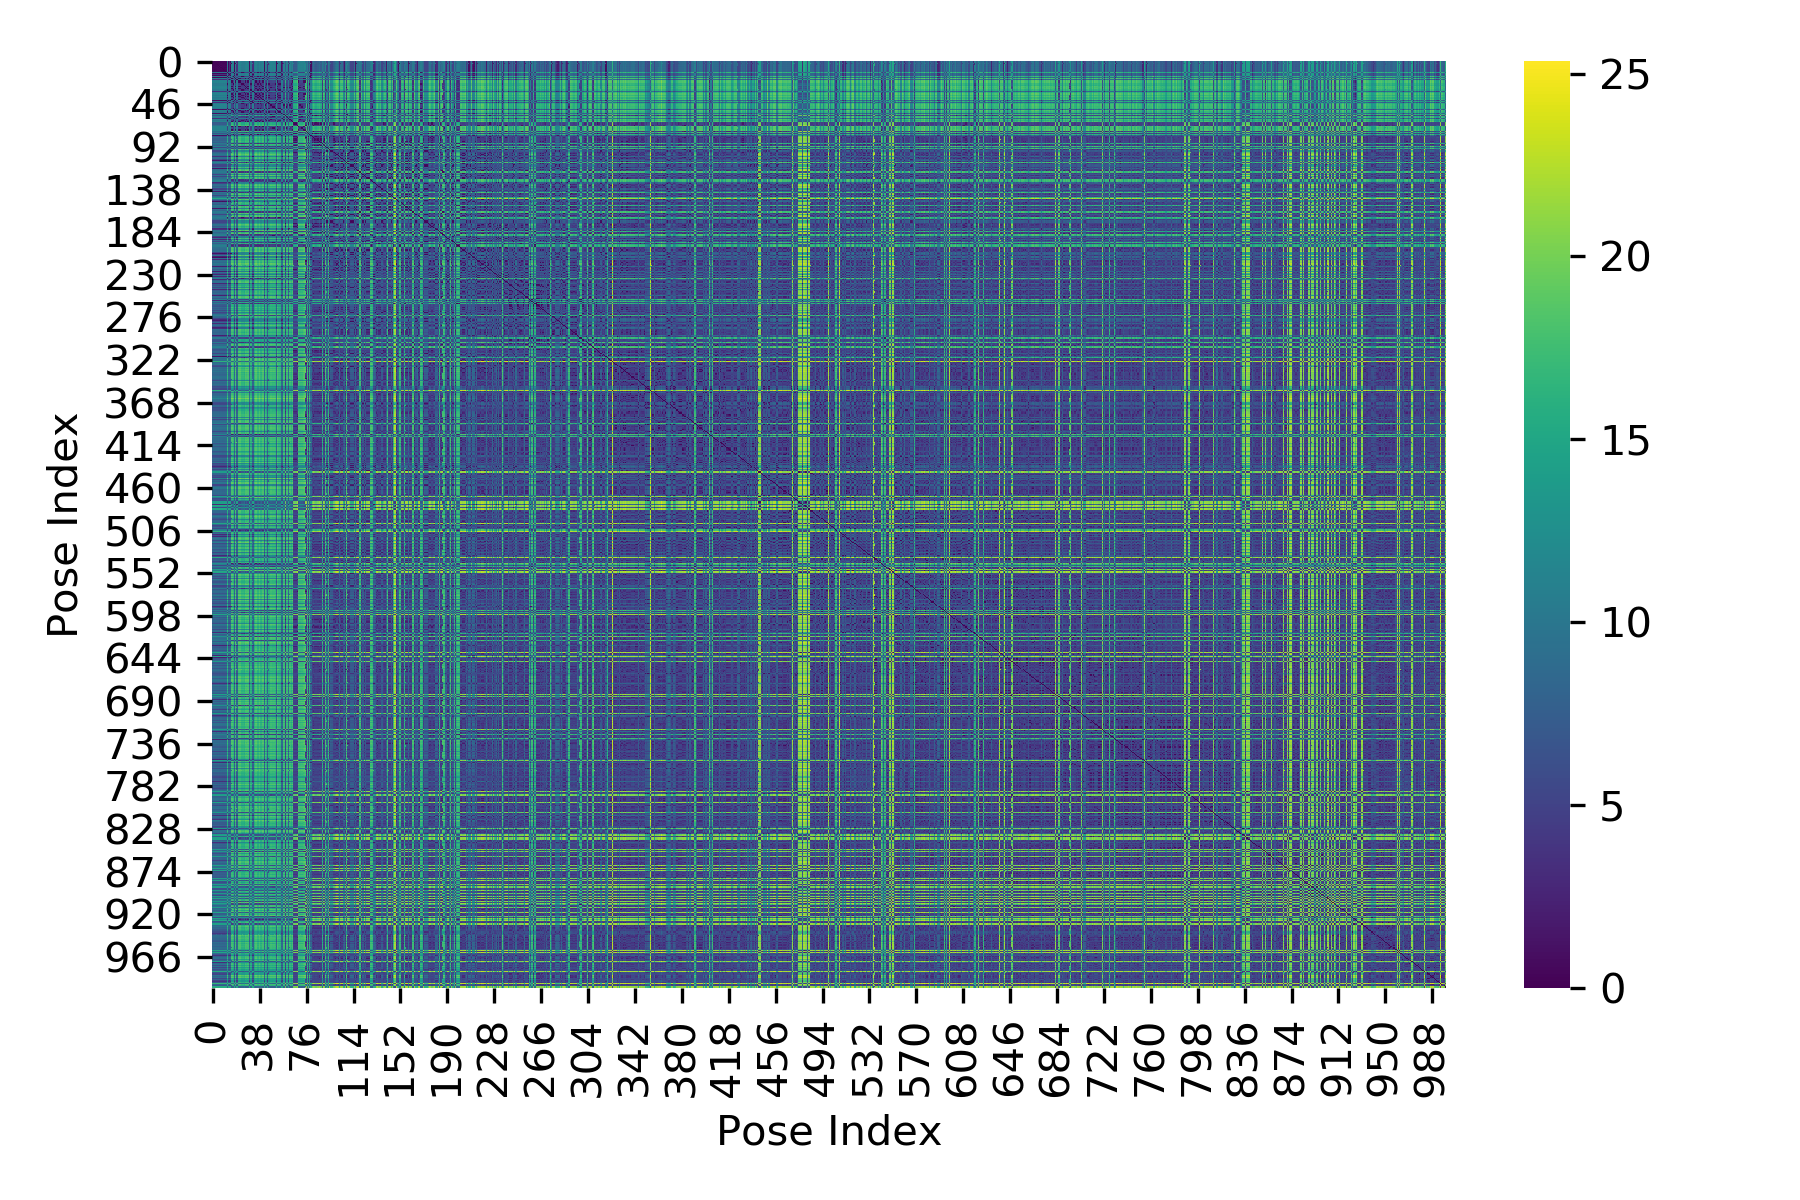
\includegraphics{chapter6/Figures/GVG_1-rmsd_matrix.png}
    \caption[RMSD Similarity Matrix]{RMSD {\AA} similarity matrix from 1000 docked poses for GVG1. Poses which are similar will have a low RMSD represented by darker colors (blue to purple) and poses which are dissimilar will have a high RMSD represented by brighter colors (green to yellow). This shows the raw similarities between docked poses.}
    \label{fig:similarity_matrix}
\end{figure}

First, we generate a RMSD-based similarity matrix of the 1000 generated docked poses.
That is, we compute the RMSD, using only the ligand heavy atoms, from each docked pose to every other docked pose.
This gives us an $N x N$ similarity matrix (N=1000), in which our measure of similarity is based on the calculated RMSD between the docked poses (Fig. \ref{fig:similarity_matrix}).
Next, we apply a technique called Multi-Dimensional Scaling (MDS) through scikit-learn (v0.19.0) \cite{scikit_mds} in order to reduce our $N x N$ dimensional space into a 2D space, where we can then apply clustering techniques.
MDS is a method which transforms our similarity matrix and projects each object (i.e pose) into a lower dimensional space in such a way that the distance between objects (i.e poses) are preserved as best as possible.
In other words, when we project into a 2D space, poses which are similar (low RMSD) will appear closer together and poses which are dissimilar (high RMSD) will appear farther away.

\begin{figure}
    \centering
    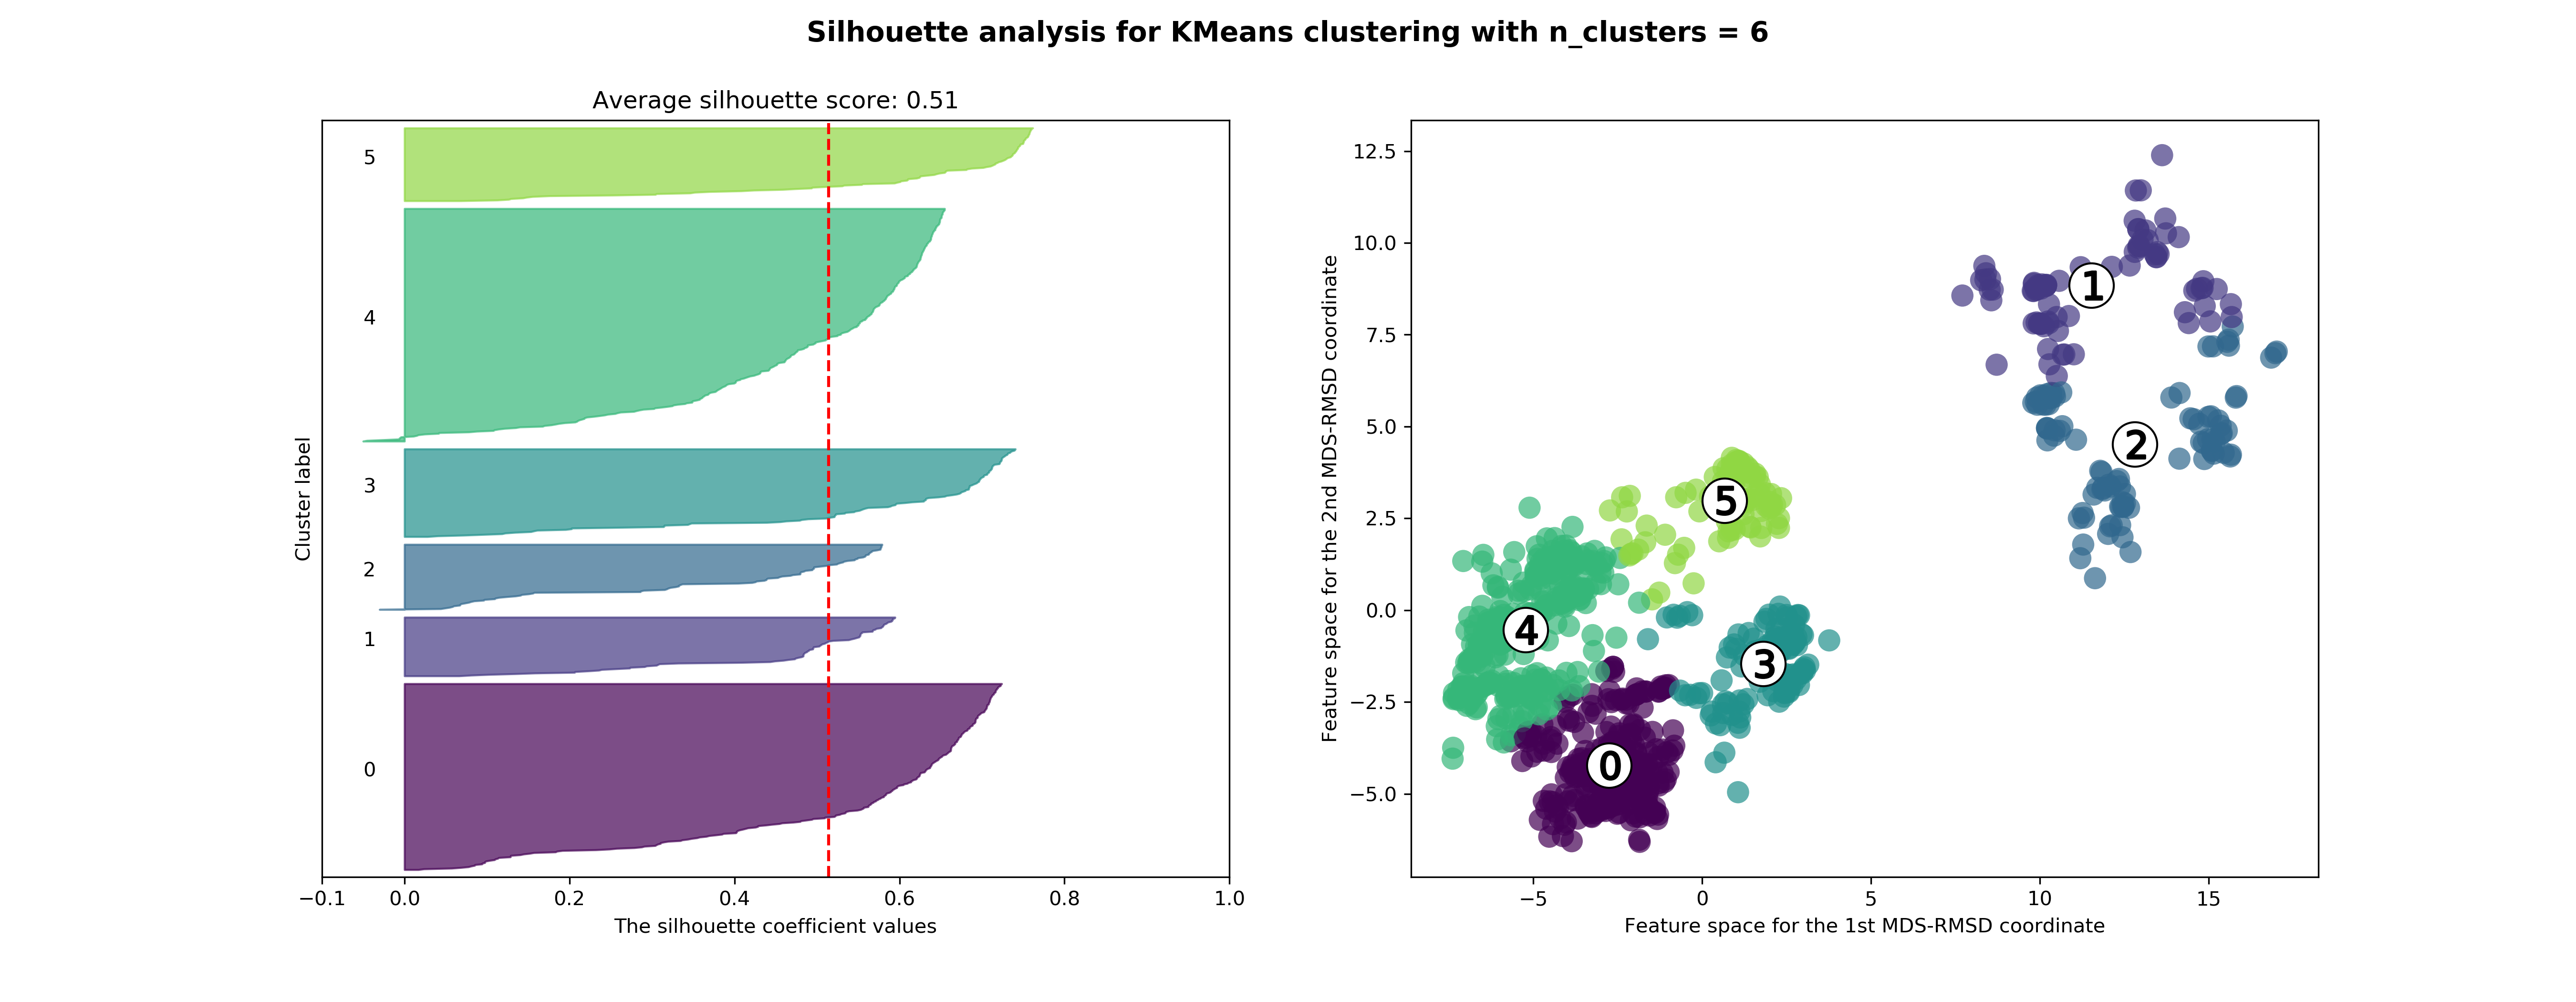
\includegraphics{chapter6/Figures/GVG_1-mds_6.png}
    \caption[Silhouette scoring in MDS-RMSD space]{Left: Silhouette scores from 1000 docked poses for GVG1 using 6 clusters from K-means clustering. Right:MDS-RMSD scatter plot for 1000 docked poses for GVG1 with K-means clustered points using 6 clusters. The cluster centroids are denoted by a number in white circles.}
    \label{fig:mds}
\end{figure}

After applying MDS to our RMSD similarity matrix, we transform our $N x N$ dimensional space and take our first two MDS components to project the data into a 2D scatter plot.
This enables us to easily apply K-means clustering \cite{scikit_kmeans} (from scikit-learn) to group up similar poses and separate dissimilar poses with the first two components which best represent the pair-wise similarity distances.
A notable downside to K-means clustering is that one has to specify the number of clusters to be used to separate the data points.
To avoid bias, we use silhouette scoring \cite{scikit_silhouette} (from scikit-learn) to automatically determine the best number of clusters to use to separate our data points.
Silhouette scoring is a method which ranges from -1 to +1 and evaluates how similar objects belonging to the same cluster are (cohesion) and how dissimilar those objects are with other clusters (separation) (Left: Fig. \ref{fig:mds}).
High values (closer to +1) indicate that the object is similar to other objects within the same cluster and dissimilar to objects in neighboring clusters.
Low values (closer to -1) indicate that the object is dissimilar to others within the same clusters and similar to objects in neighboring clusters.
A low total silhouette score indicates that the clustering configuration is likely incorrect with either too many or too few clusters, so we can use the total silhouette score as a way to select the optimal number of clusters.

We apply K-means clustering using a range of 2-9 (K) clusters on our MDS-RMSD scatter plot and score each round of clustering using silhouette scores.
We selected the number of clusters K maximizing total silhouette score, and then used this to partition our 1000 docked poses in MDS-RMSD space and set the number of starting poses to be used for our simulations.
Using the K clusters which maximized the silhouette score, we then selected the centroid of each cluster as the representative pose for starting our simulations (Right: Fig. \ref{fig:mds}).

\subsection{Molecular Dynamics and BLUES Simulations}
In this study, we used two simulation approaches: traditional molecular dynamics (MD) simulations and our hybrid approach called BLUES: Binding modes of Ligands Using Enhanced Sampling \cite{BLUES_paper}, which combines Non-equilibrium Candidate Monte Carlo (NCMC) \cite{ncmc_paper} move proposals with MD.
Both MD and BLUES simulations using OpenMM (v7.1.1) \cite{openmm} with the same solvated SEH system.
For our simulations, the truncated SEH protein (consisting of only the C-terminal domain) was paramterized with amber99sbildn forcefield for the protein and GAFF2 for the ligands, and solvated with TIP3P waters \cite{lindorff-larsen_improved_2010}.

We performed a maximum of 30,000 energy minimization steps and a 3 stage (NVT, NPT, NPT) equilibration protocol which we describe as follows.
In each equilibration stage, a restraint force is placed on the $\alpha$-Carbons of the protein backbone and the ligand heavy atoms, where we successively decrease the force from $2.0 \frac{kcal}{mol \cdot \mbox{\AA} ^{2}}$ to $0.5 \frac{kcal}{mol \cdot \mbox{\AA} ^{2}}$ to $0.1 \frac{kcal}{mol \cdot \mbox{\AA} ^{2}}$ at each stage.
After equilibration, we ran 1 microsecond ($\mu$s) using molecular dynamics (MD) and 600 nanoseconds (ns) using BLUES for each pose selected by our MDS-RMSD filtering protocol (described in the previous section).
Our simulations were run using 4 femtosecond (fs) timesteps and with the hydrogen-mass repartioning scheme \cite{hmass_repartition}.

Briefly, we describe our protocol for BLUES simulations.
A BLUES simulation begins with the NCMC phase, which involves proposing a random rotation about the ligand center of mass and then relaxes via a series of non-equilibrium switching steps which alchemically scale the ligand interations off/on over $N$ steps.
This is in contrast to traditional Monte Carlo, which involves performing an instantaneous change to the ligand coordinates.
Specifically, interactions are controlled via a parameter ($\lambda_{0 \rightarrow 1}$) which scales the ligand interactions with the surrounding environment.
Our non-equilibrium switching protocol begins with the fully interacting ligand at $\lambda_{0}$ and then we alchemically scale the ligand forces off until $\lambda_{0.5}$, where the ligand is no longer interacting with surrounding atoms.
We perform the proposed random rotation on the non-interacting ligand and then alchemically scale the ligand forces back on until $\lambda_{1}$, where the ligand is fully interacting and in the proposed positions.
Over the series of $N$ NCMC switching steps, we accumulate the total non-equilibrium work done and use this in acceptance or rejection of the proposed move (following the Metropolis-Hasting acceptance criterion \cite{met_hastings_acceptance}).
After the Metropolization step, we follow-up using traditional MD methodology and repeat the cycle (NCMC -> MD -> NCMC...etc.) for $I$ iterations.

\subsection {Determination of Binding Modes with TICA and PCCA}
We divide the SEH binding site (Figure \label{fig:truncated-protein}) into two sub-cavities denoted as ``left'' and ``right'' and analyze simulation data from these two sub-cavities separately, as we rarely observed transitions between them.
That is, simulations which started with dock poses in the right sub-cavity were pooled together and vice versa, but simulations in each sub-cavity were kept separate, since very few simulations exhibited transitions and thus pooling data across sub-cavities would have complicated analysis.
By treating the two sub-cavities separately, we are better able to distinguish between binding modes sampled within each sub-cavity and understand their timescales, over the timescale to transition between sub-cavities.
In other words, we can better distinguish rapid transitions between binding modes within each sub-cavity over the slow transitions between sub-caivities.
Additionally, if we had pooled together simulation data from both sub-cavities, our silhouette scores would always suggest 2 binding modes, which is actually just the separation of binding modes between the two cavities.

\begin{figure}
    \centering
    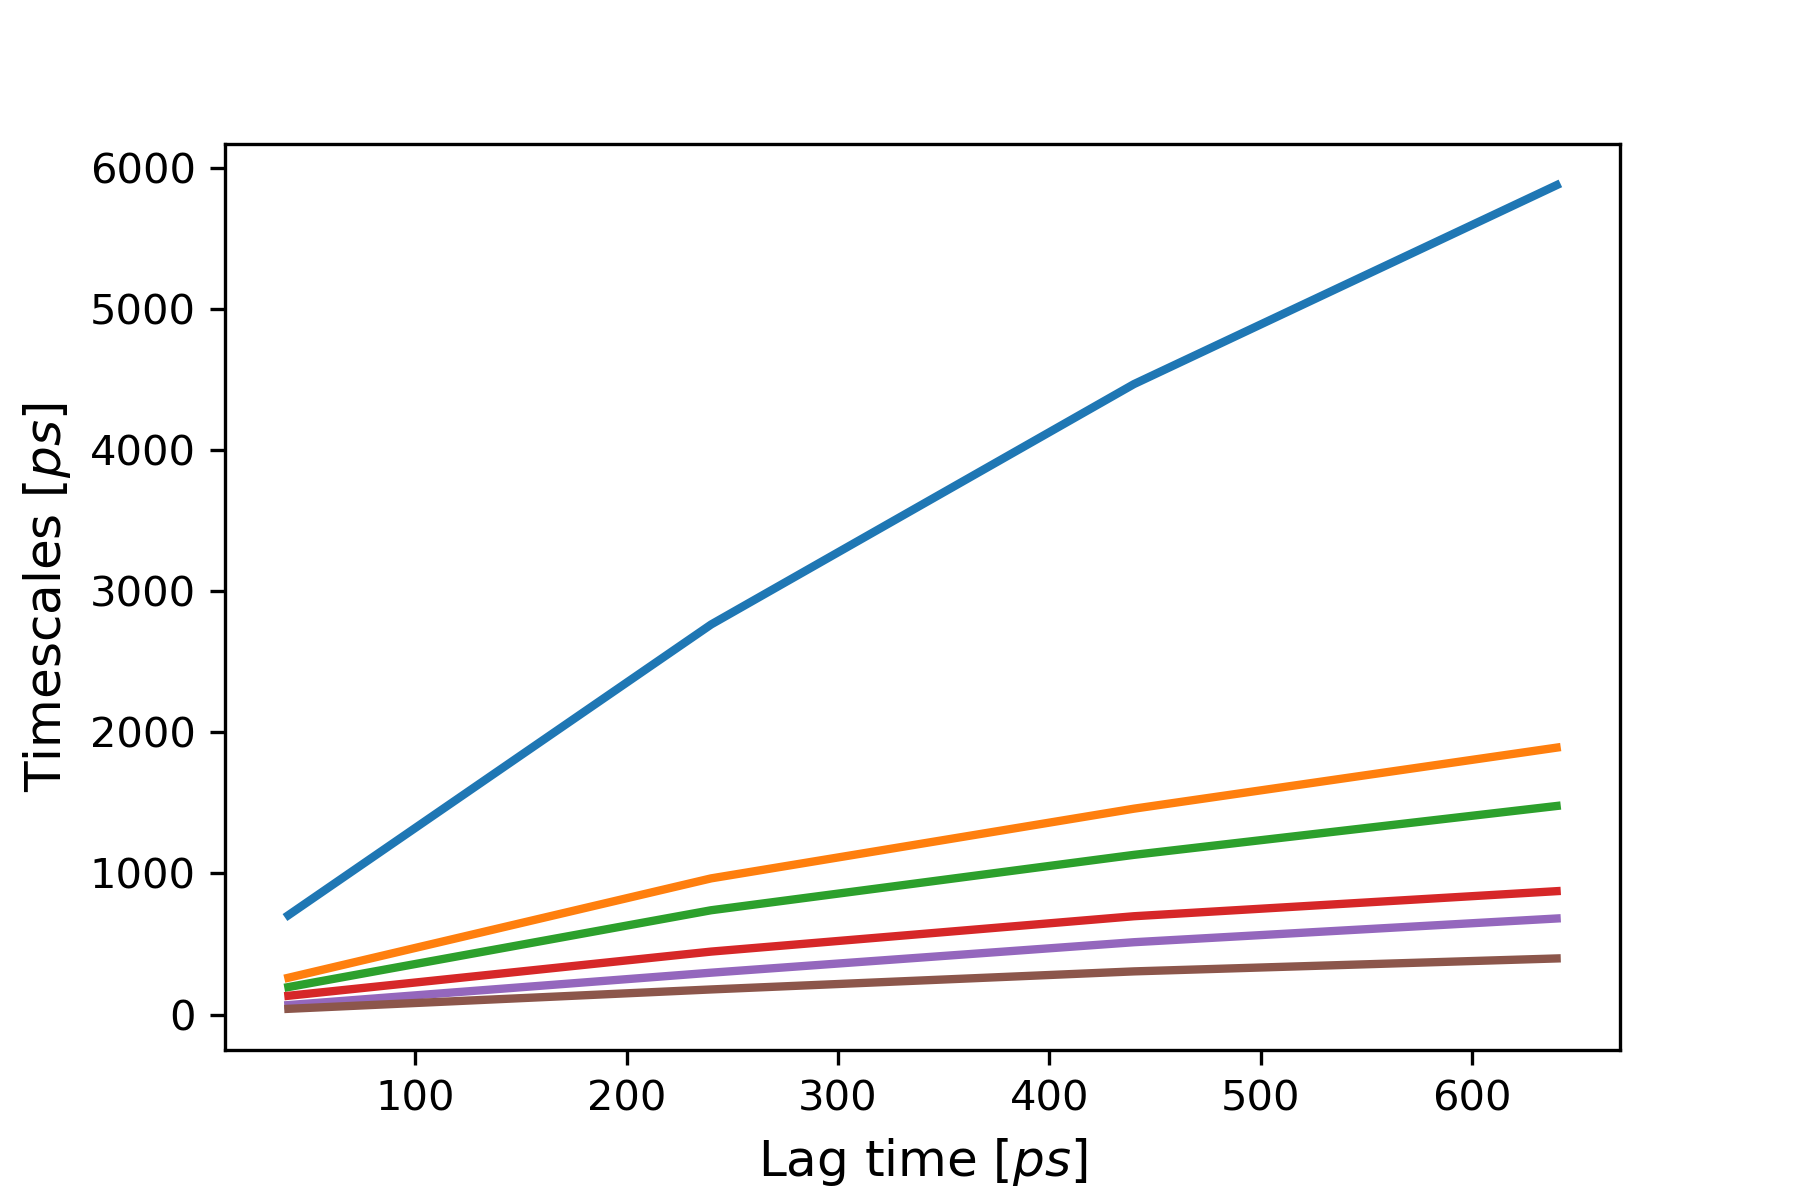
\includegraphics{chapter6/Figures/GVG_1-right_imptimescales.png}
    \caption[Implied Timescales for GVG1]{Implied timescales plot for GVG1 from our BLUES simulatinos. This plots a series of lag times (picoseconds) versus timescales of various states. The choice of lagtime to discretize our simulation frames was chosen by selecting a lagtime where it begins to become independent of timescales. We chose a lagtime of 400ps.}
    \label{fig:GVG_1-right-imptimescales}
\end{figure}

Using PyEMMA (v2.5.5), we analyzed and built Markov State Models (MSM) separately between our MD and BLUES simulations.
MD simulation frames were stored every 25,000 steps (100ps/frame) and BLUES simulation frames were stored every 10,000 steps (40ps/frame).
In this study, we apply a method called time-lagged indepdent component analysis (TICA) with perron-cluster cluster analysis (PCCA) to define our metastable binding modes sampled during our simulation.
The appropriate lagtime for TICA was chosen by plotting the implied timescales versus a series of lagtimes and selecting a lagtime where the timescales appeared to be independent of lag time (Figure \ref{fig:GVG_1-right-imptimescales}).
Here, $N$ is defined as the square root of the total number of simulation frames, which is the default choice for PyEMMA.
We used lagtimes of 250ps for MD and 400ps for BLUES simulations.

\begin{figure}
    \centering
    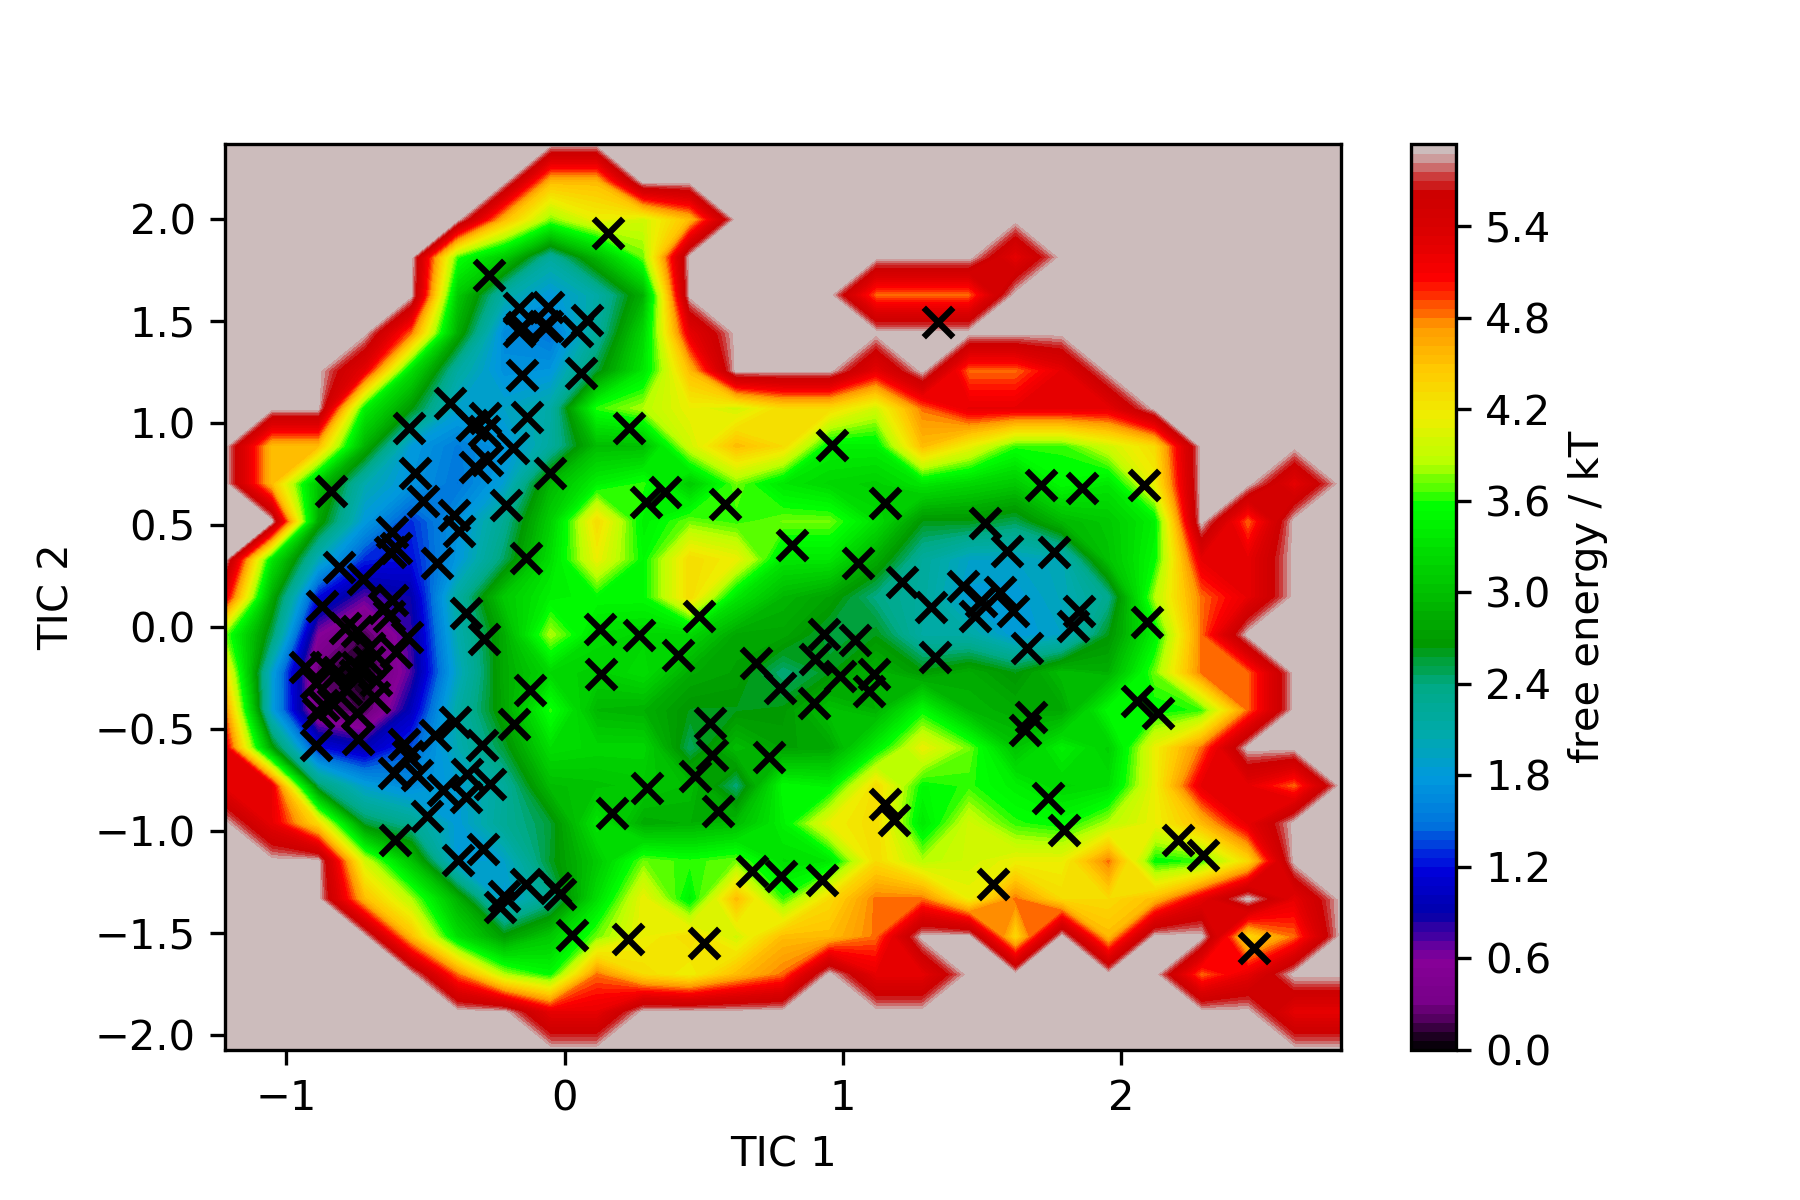
\includegraphics{chapter6/Figures/GVG_1-right_c4-tica.png}
    \caption[TICA plots for GVG1]{Time-lagged indepdent component analysis (TICA) plot for binding modes of GVG1 located in the right sub-cavity using the first two TICA components. Discrete microstates (i.e. simulation frames are denoted by black Xs. Metastable states sampled during the simulation are indicated in darker colors (blue-purple) in the contours or where Xs are more dense.}
    \label{fig:GVG_1-right-tica}
\end{figure}

\begin{figure}
    \centering
    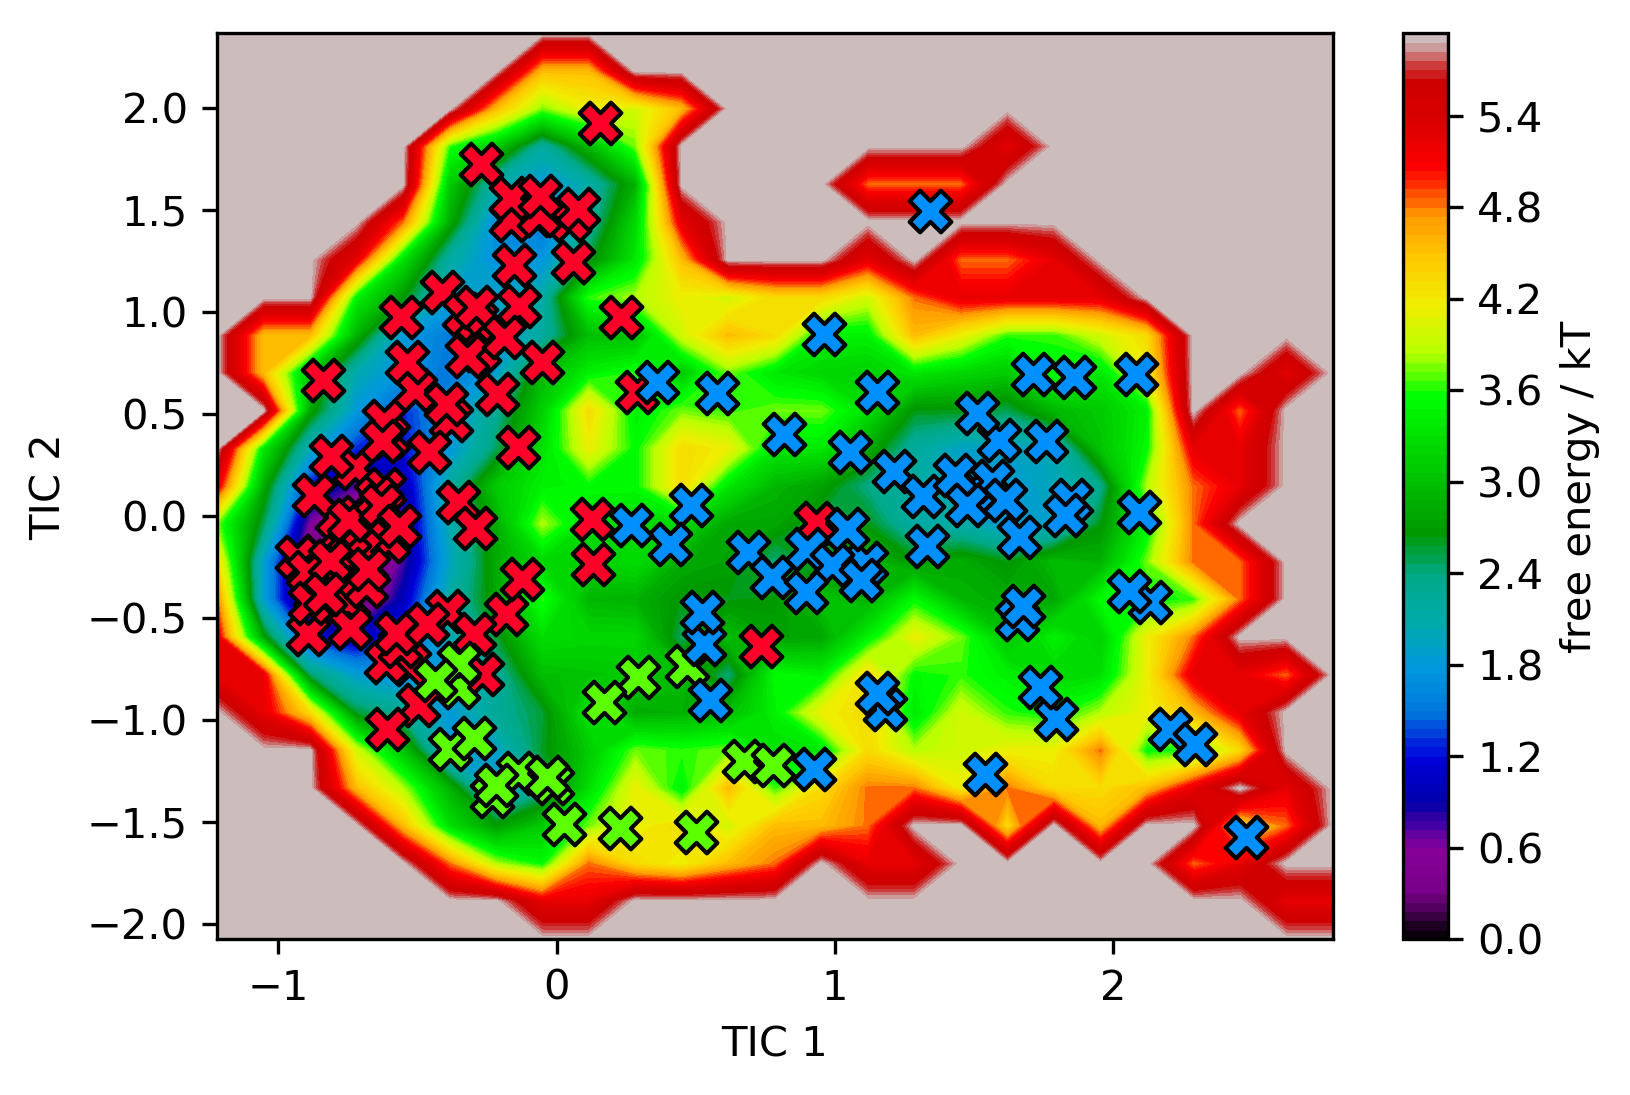
\includegraphics{chapter6/Figures/GVG_1-right-pcca.png}
    \caption[PCCA plot for GVG1]{TICA plot for binding modes of GVG1 located in the right sub-cavity using the first two TICA components. Each X denotes a discrete microstate (i.e. simulation frame). Each microstate has been assigned to a macrostate by PCCA which define our metastable binding modes sampled during our simulation. We find 3 states (red, green ,blue) or binding modes sampled from simulations of GVG1 in the right sub-cavity.}
    \label{fig:GVG_1-right-pcca}
\end{figure}

In this study, we analyzed the distances between the ligand heavy atoms and each of residues ASP110, TYR158, MET194, TYR241 and VAL273.
These were chosen because they were highlighted in an experimental study as being key residues for binding (\cite{lotz_unbiased_2018}).
With these distances to key residues as our feature set, we applied TICA \cite{perez-hernandez_identification_2013} to extract the slow order parameters and mapped our simulation frames via k-means clustering.
This gives us a set of $N$ discrete microstates (i.e. simulation frames) into the coordinate space of the first 2 TICA components (Fig. \ref{fig:GVG_1-right-tica}).

In Figure \ref{fig:GVG_1-right-pcca},  we define our macrostates or metastable binding modes, by assigning each microstate to a given $K$ number of macrostates via PCCA \cite{roblitz_fuzzy_2013,deuflhard_robust_2005}.
To determine the appropriate number of $K$ macrostates to use, we evaluate the clustering using silhouette scoring \cite{scikit_kmeans} (discussed previously).
In our analysis we represent each macrostate by randomly draw 100 simulation frames from the pool of microstates assigned to each $K$ macrostates.

In Fig \ref{fig:GVG1_c4-md}, we plot the RMSD of the ligand heavy atoms relative to the starting configuration and color each time point by assigning it to the macrostate which minimizes the RMSD.
Specifically, we compute the ligand heavy atom RMSD to the 100 representative microstates (simulation frames) belonging to each macrostate; then, assign it to the macrostate which minimizes the RMSD.
We can then compute the populations or amount of simulation time spent within each binding mode by counting the membership assignment of the simulation frames.

\subsection {Crystallographic Binding Mode Predictions}
To evaluate the ability to predict dominant binding modes as determined by crystallography using docking, MD, or BLUES, we report two RMSD ({\AA}) metrics: an `averaged' RMSD and the minimum RMSD.
Here, our reported average RMSD is calculated by averaging over 10,000 randomly drawn (with replacement) values from the remaining (MDS-RMSD filtered) docked poses or 100 simulation frames which we saved to represent each binding mode.
We believe this `average' RMSD best represents random selection of a single docked pose from a pool of poses or a single frame from the whole simulation to compare against the crystallographic structure.
We also report the minimum RMSD as this represents the best case or `ideal' scenario where we could identify which structure generated from docking or sample from our simulations would be closest to the crystallographic binding mode. H
owever, we are not aware of any method which could identify such poses so we view minimum RMSD to be useless as a performance metric.
Here, we include it simply to provide a way to assess whether any poses were sampled that were close to the crystallographic bining mode.

We remind the reader that our analysis treats each sub-cavity \ref{fig:truncated-protein},  separately.
There were a total of 29 crystallographic binding modes to be identified out of the 12 ligand we simulated, where molecules fell into 2 groups: those with a single binding mode and those with multiple binding modes (2+).
For ligands with a single binding mode, we report the average and minimum RMSDs (described previously) of the ligand atoms in the crystallographic structure against those in the representative frames from the binding mode with the highest occupancy (i.e simulation time).
When ligands have multiple crystallographic binding modes, we report the lowest RMSD from the binding modes found from simulations, relative to each crystallographic binding mode.
We describe a successful prediction as being within 2 {\AA} of the crystallographic binding mode and close predictions as predictions within 4 {\AA} of the crystallographic binding mode.

\section{Results}
Here, we analyze the success of docking, standard MD and BLUES at recovering crystallographic binding modes of a series of 12 ligands which have a total o 29 binding modes between them.
In our analysis, we consider data only from docked poses or binding modes sampled during our simulations which are in the correct sub-cavity.
That is, if the crystallographic structure was found in the right sub-cavity, we computed the RMSD using docked poses or simulation frames that were only in the right sub-cavity (and vice versa).
In this study, we consider predictions successful when they are within 2 {\AA} of the crystallographic binding mode and we label predictions ``close'' when they are within 4 {\AA}.
There were a total of 29 binding modes to be predicted from our set of 12 molecules simulated.

We remind the reader that we report an `averaged' RMSD from each method (See Methods:Comparison to the crystallographic pose).
Since we cannot determine which docked pose or single simulation frame would result in minimizing the RMSD to the crystallographic binding mode without bias, an averaged RMSD represents randomly picking from a pool of docked poses or a single simulation frame representative of a metastable binding mode.
Note, the reported RMSD from docking is representative of the remaining docked poses after applying our RMSD-MDS filter to the initial pool of 1000 generated docked poses.
Here, we will also report the minimum RMSD to show the best case or `ideal' scenario for each method.
The minimum RMSD reflects the performance which would be expected if one could determine somehow, without knowing the crystal structure, which docked pose or simulation frame would be closest to the true binding mode.

\begin{figure}
    \centering
    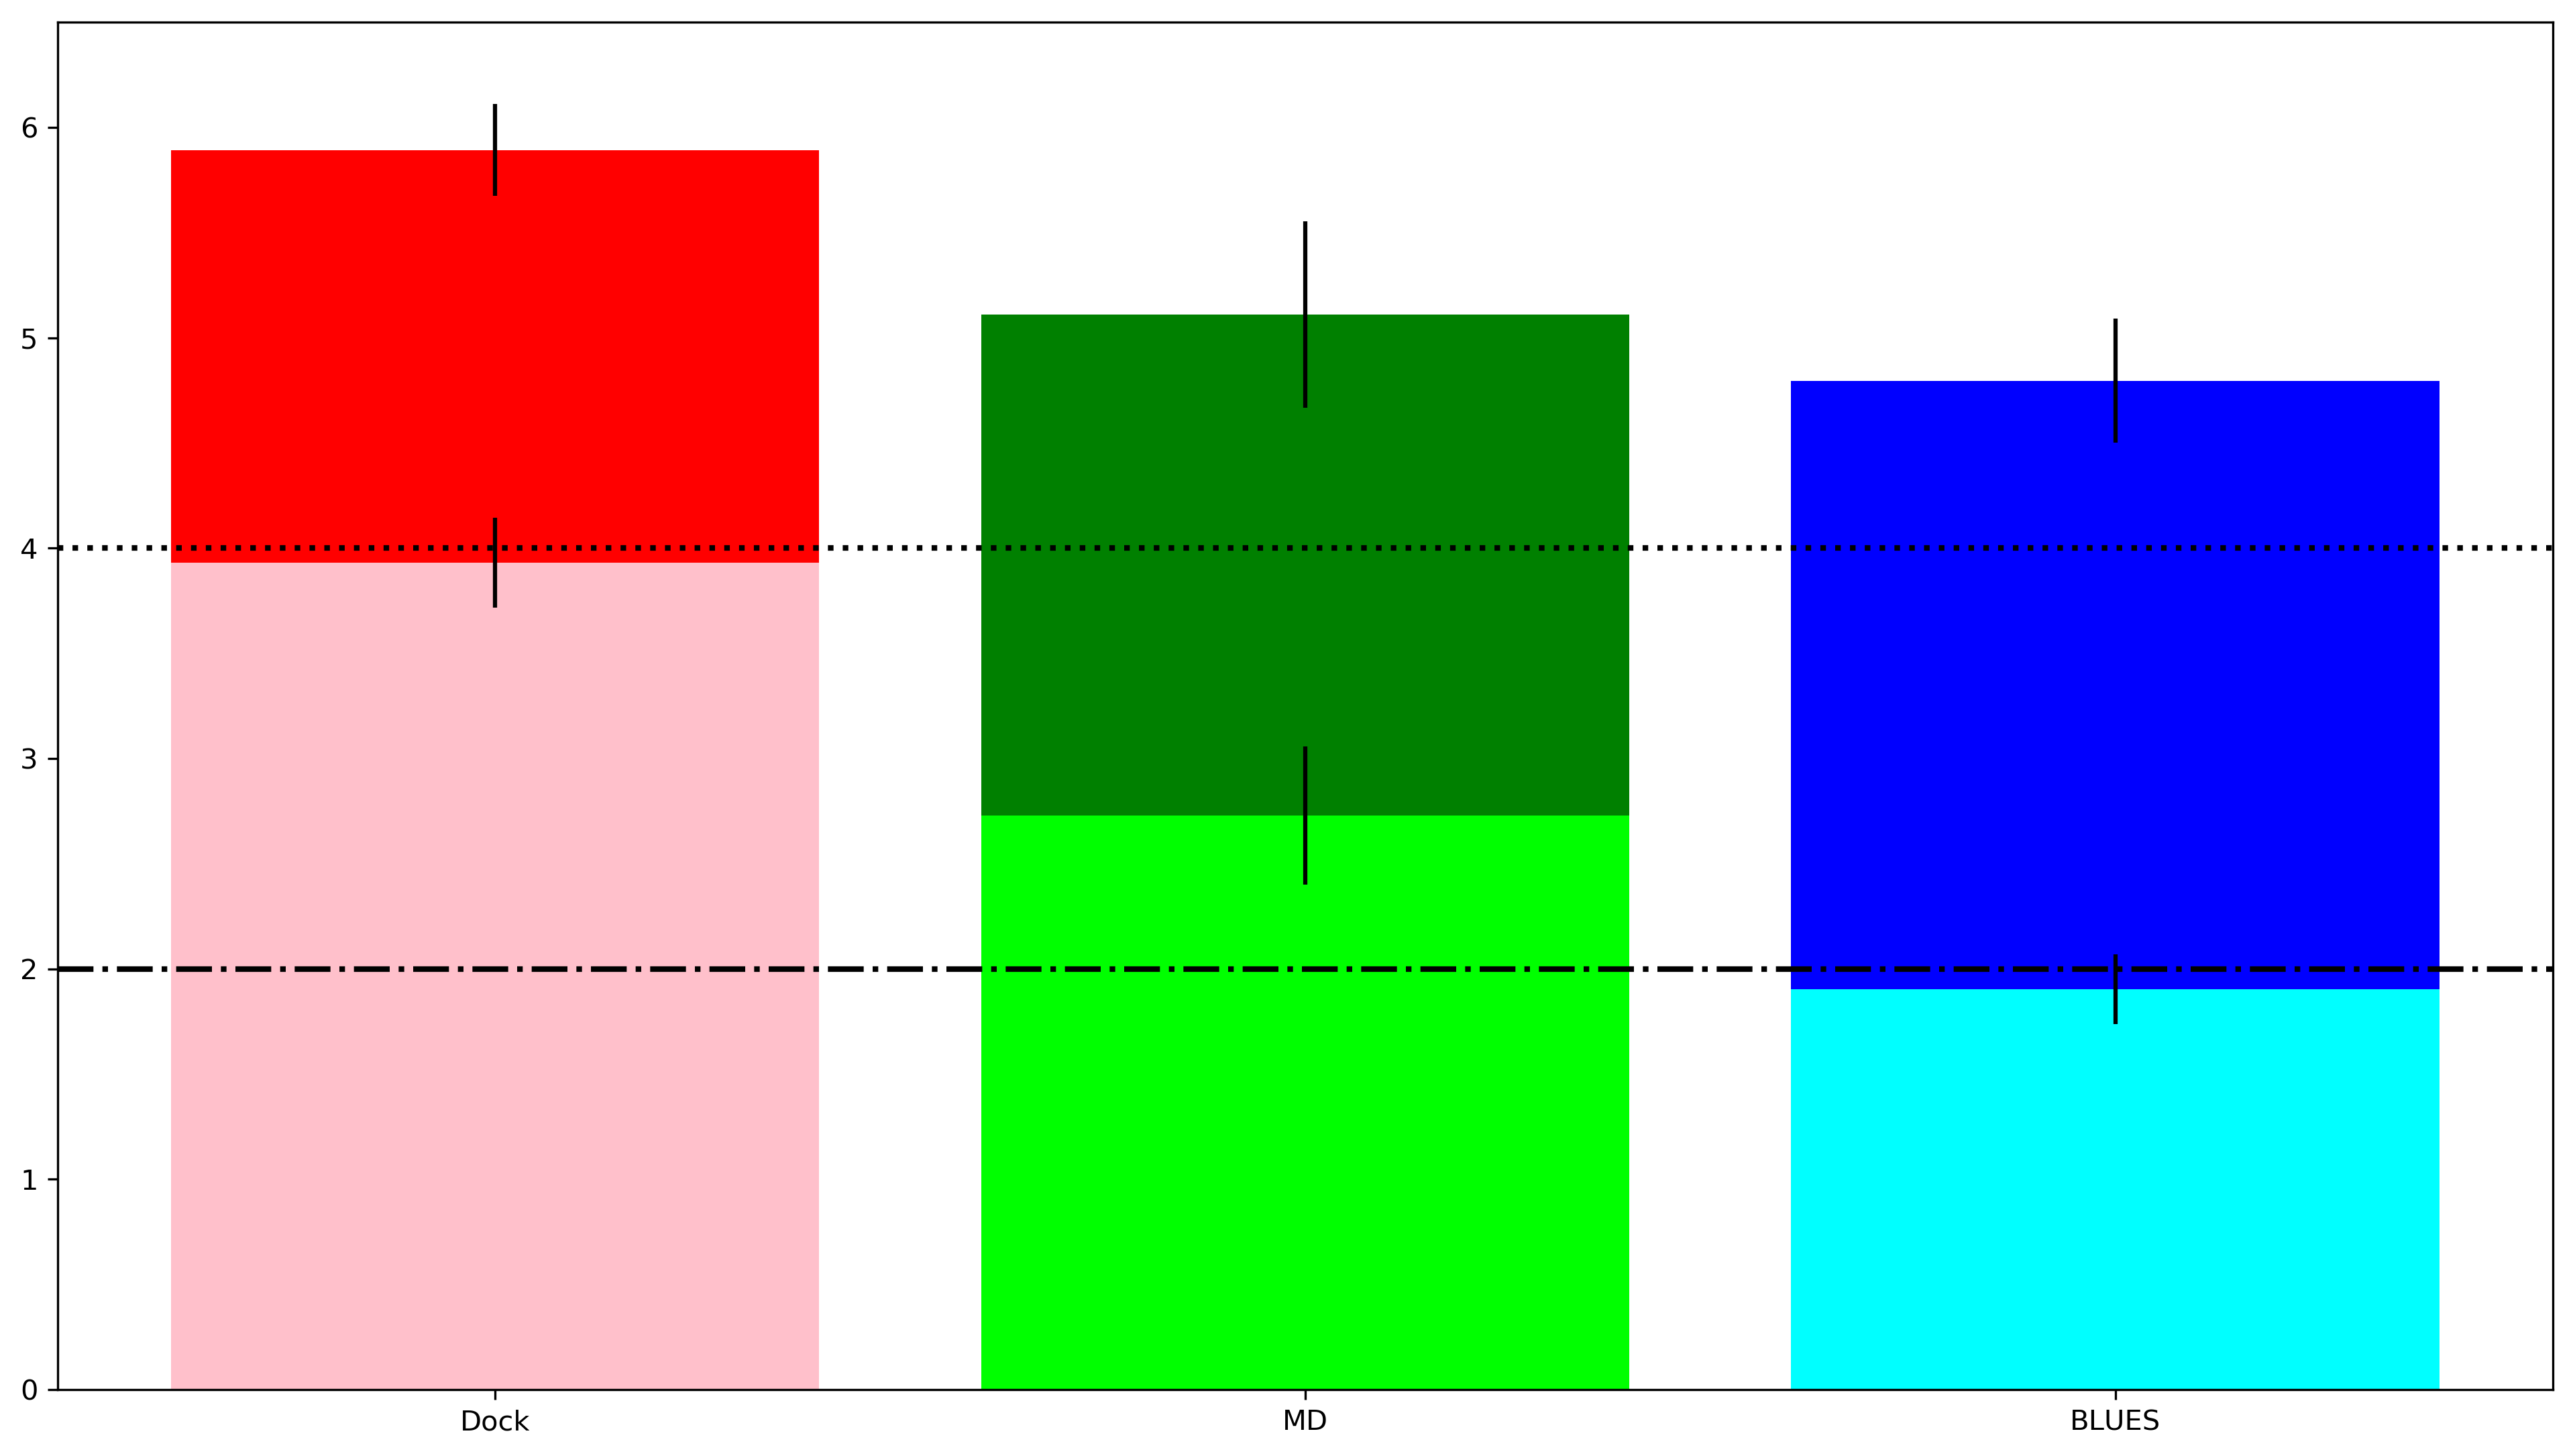
\includegraphics{chapter6/Figures/averages.png}
    \caption[Average RMSD]{Minimum/Average RMSD for each method: docking (pink/red), MD (lime/green), and BLUES (cyan/blue) for all ligands in this study. Dashed line at 2 {\AA} represents successful predictions and dotted line at 4 {\AA} represents close predictions. This reports the averaged RMSD from all 12 ligands used in this study.}
    \label{fig:averages}
\end{figure}
Here, we find that no method always correctly identifies the crystallographic binding mode (as evidenced by average RMSD) but both MD and BLUES substantially outperform docking at sampling binding modes near the crystallographic one, and of these, BLUES performs better.
Averaged across all of the ligands in this study,  the minimum RMSDs for docking (pink), MD (lime), and BLUES (cyan) were $3.9 \pm 0.2 {\AA}$, $2.7 \pm 0.3 {\AA}$, and $1.9 \pm 0.2 {\AA}$ respectively; the average RMSD for docking (red), MD (green), and BLUES were $5.9 \pm 0.2 {\AA}$, $5.1 \pm 0.4 {\AA}$, and $4.8 \pm 0.3 {\AA}$ respectively ( (Fig. \ref{fig:averages}).

On average, when considering both cases of single and multiple crystallographic binding modes to identify, none of the 3 methods considered here appear to make predictions which are close (within 4 {\AA}) to the crystallographic binding mode.
Across the dataset, both BLUES and MD were able to identify the crystallographic binding mode in 2/29 cases when considering the average RMSDs and none from docking.
If we consider the ideal scenario--that is, considering the minimum RMSD--docking will make predictions which are within 4{\AA} of the crystallographic binding mode, with some improvement in RMSD via MD simulation.
At best (considering the minimum RMSD), BLUES predictions may be within at least within 2 {\AA} to the crystallographic binding mode.
Across the dataset, considering the minimum RMSDs, docking can identify 2/29 (7\%) binding modes, MD can identify 11/29 (38\%) binding modes and BLUES can identify 16/29 (55\%) of the binding modes.
This suggests that BLUES does better than MD and docking at sampling near the crystallographic binding mode.

\subsection{Analysis of Molecules with a Single Binding Mode}

\begin{figure}
    \centering
    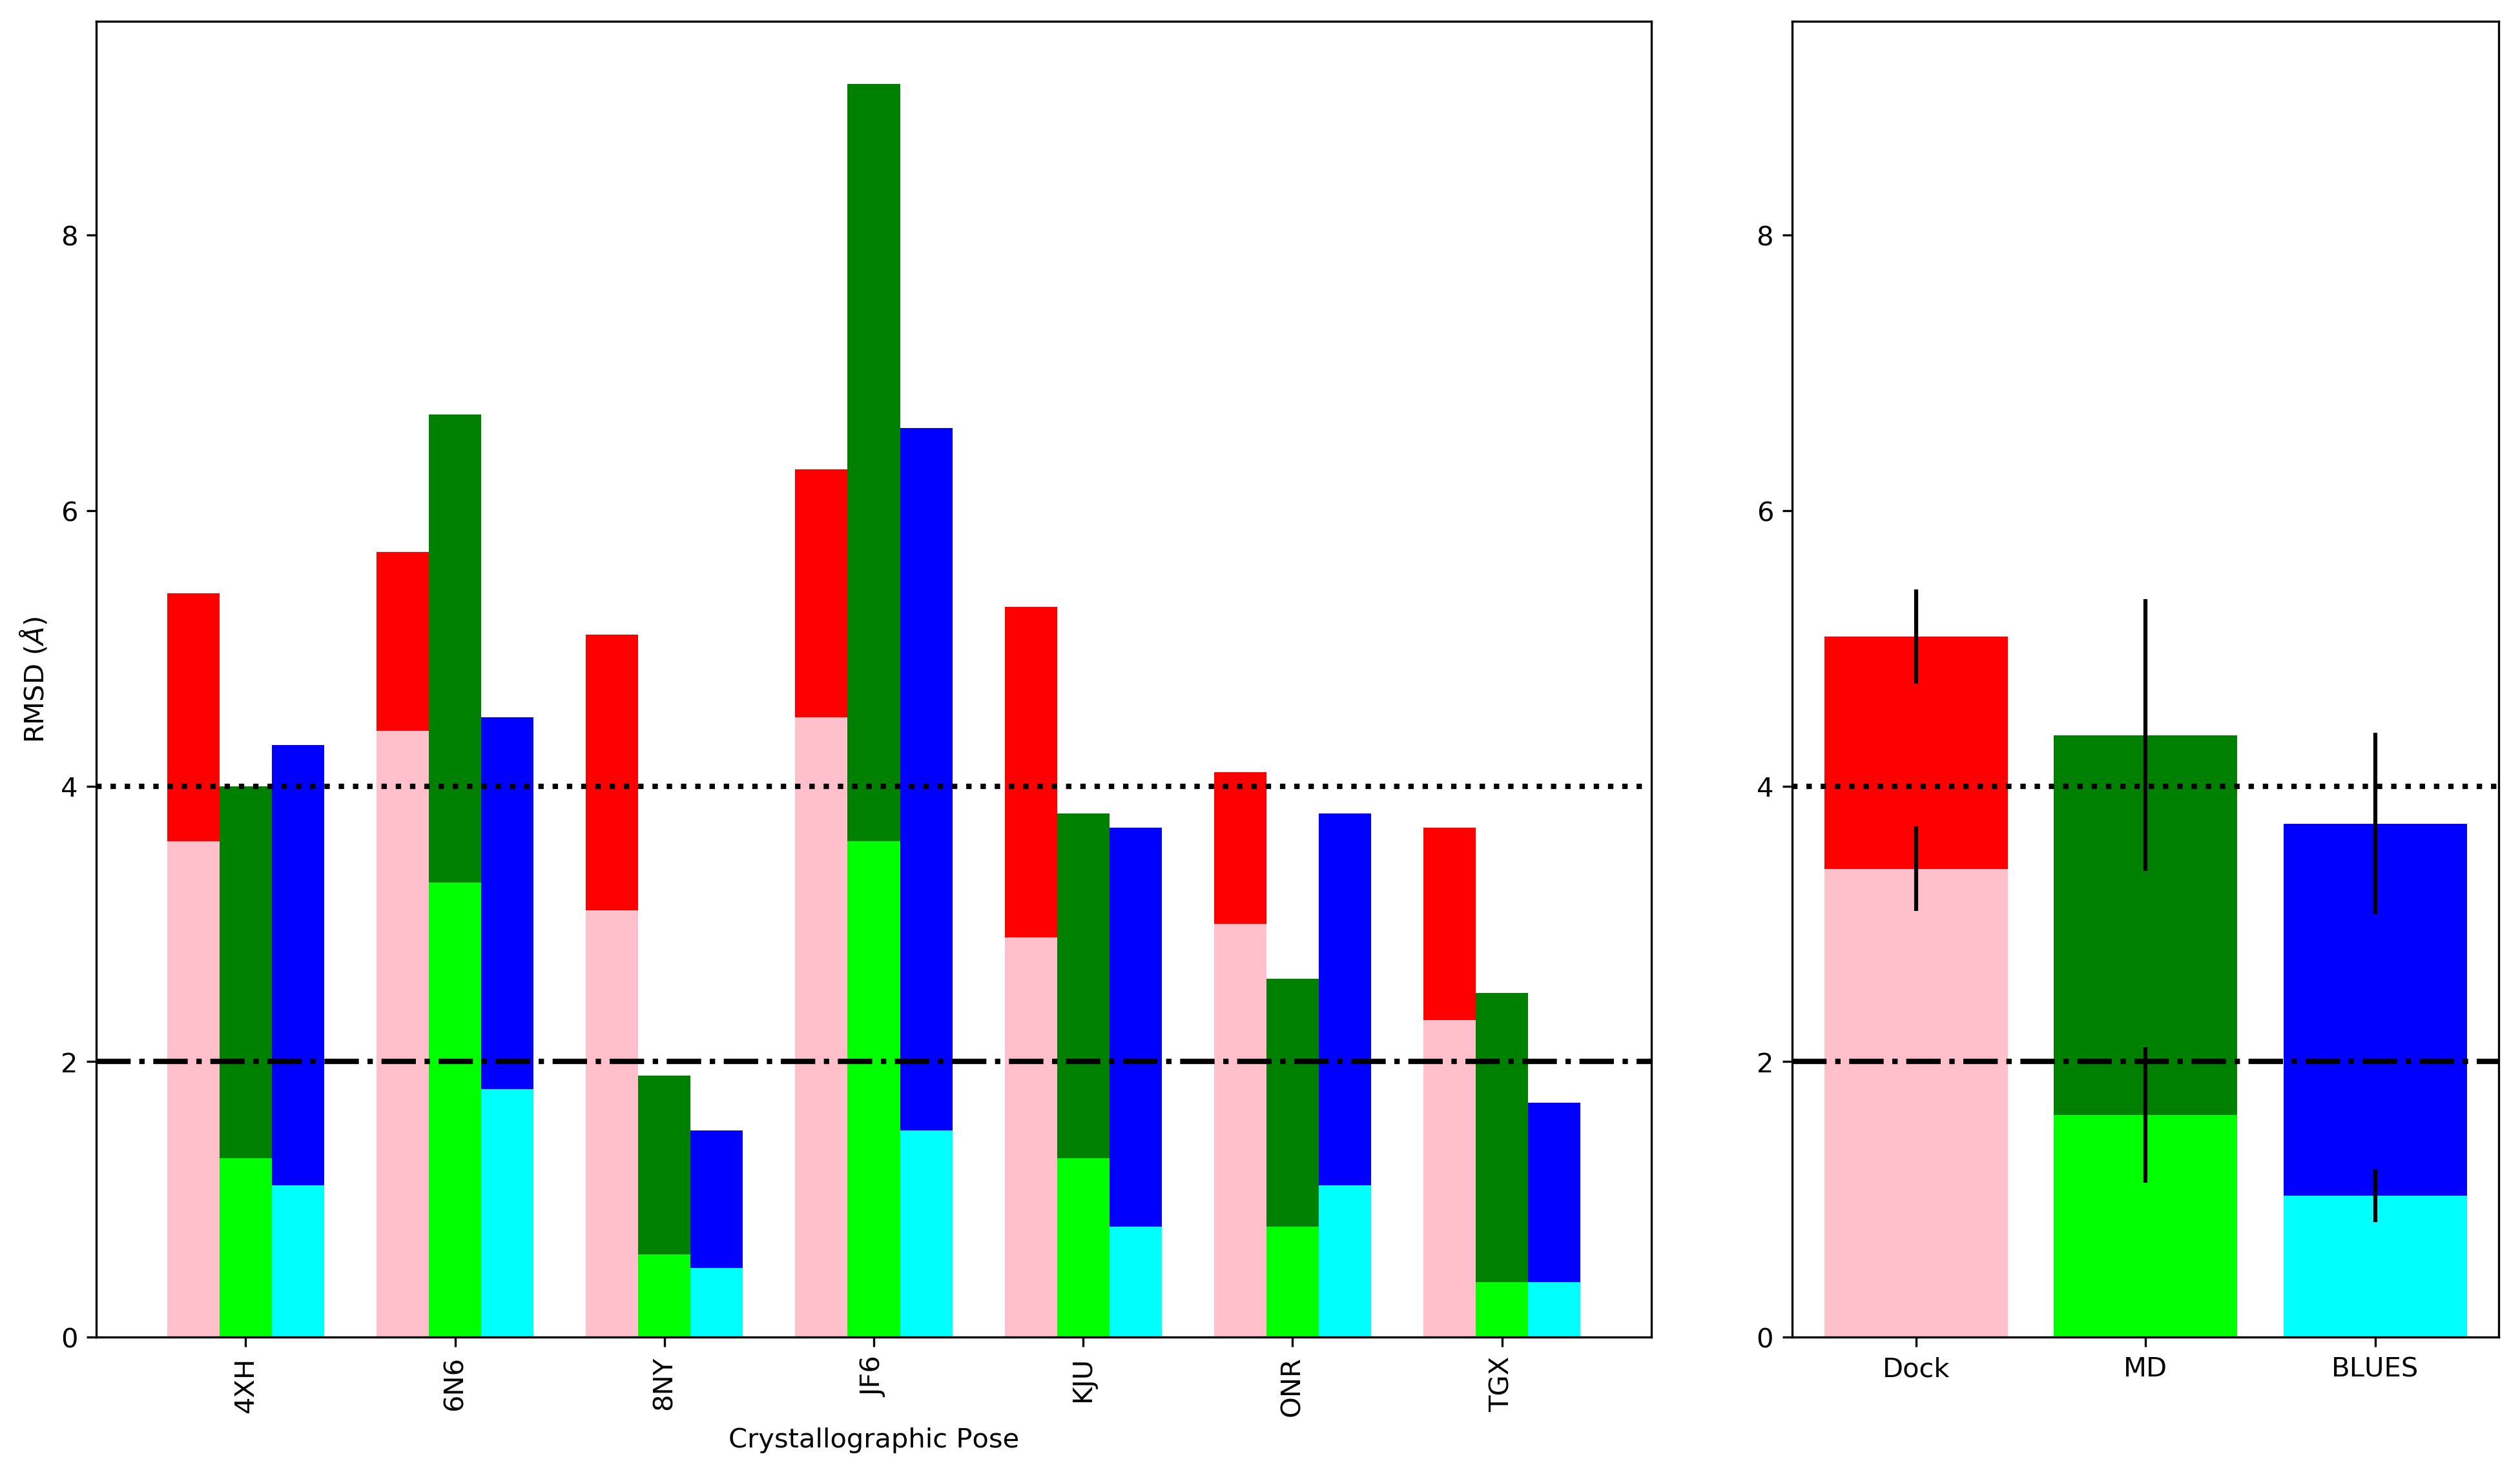
\includegraphics{chapter6/Figures/singlebm.png}
    \caption[Single Binding Mode RMSD]{Left: Calculated RMSDs (minimum/average) relative to the crystallographic ligand binding mode and binding modes from docking (pink/red), MD (lime/green), and BLUES (cyan/blue) simulations for ligands with a single binding mode. Successful prediction in binding mode is judged to be less than or equal to 2 {\AA} (black dashed horizontal line). Right: Averaged RMSD for each method: docking, MD, and BLUES for ligands with a single binding mode. Considering the minimum RMSD averaged across ligands with a single binding mode, MD and BLUES can both make predictions with 2{\AA} to the true binding mode.}
    \label{fig:singlebm}
\end{figure}

Molecules with a single crystallographic binding mode were 4XH, 6N6, 8NY, JF6, KJU, ONR, and TGX.
Calculated RMSDs are measured in units of  {\AA} and are shown in Figure \ref{fig:singlebm}.
Docking had minimum RMSDs (pink) of 3.6, 4.4, 3.1, 4.5, 2.9, 3, and 2.3 and average RMSDs (red) of 5.4, 5.7, 5.1, 6.3, 5.3, 4.1, and 3.7.
The minimum RMSDs (lime) from the highest populated binding mode sampled during our MD simulations were 1.3, 3.3, 0.6, 3.6, 1.3, 0.8, and 0.4 with average RMSDs (green) of 4.0, 6.7, 1.9, 9.1, 3.8, 2.6, and 2.5.
From the most populated binding mode sampled during our BLUES simulations, the minimum RMSD (cyan) for each molecule was 1.1, 1.8, 0.5, 1.5, 0.8, 1.1, and 0.4 with average RMSDs (blue) of 4.3, 4.5, 1.5, 6.6, 3.7, 3.8, and 1.7.
These results indicate that BLUES performs better at sampling near the crystallographic binding mode over docking and MD.

When considering the averages (Left-Fig.\ref{fig:singlebm})--representing random selection--only predictions for 8NY from MD/BLUES and TGX from BLUES were successful in identifying the crystallographic binding mode within 2 {\AA}.
In the ideal scenario--represented by the minimum RMSDs--we see successes in 4XH, 8NY, KJU, ONR, and TGX (5/7 single binding mode cases) using MD simulations.
Using BLUES simulations, we see successes in all 7 of the single binding mode cases when considering the minimum RMSD.
On the other hand, docking had no successful predictions when considering both the minimum and average RMSD.

Across this subset of molecules with a single binding mode, the minimum RMSDs for docking (pink), MD (lime), and BLUES (cyan), were $3.4 \pm 0.3 {\AA}$, $1.6 \pm 0.5 {\AA}$, and $1.0 \pm 0.2 {\AA}$ respectively; average RMSDs for docking (red), MD (green), and BLUES (blue) were $5.1 \pm 0.3 {\AA}$, $4.4 \pm 1.0 {\AA}$, and $3.7 \pm 0.7 {\AA}$ respectively (Right-Fig. \ref{fig:singlebm}).
At best, if we consider the minimum RMSD from docking and MD, these methods can make predictions which are close (within 4{\AA}) to a single crystallographic binding mode.
On the other hand, BLUES may be able to make predictions which are within 2 {\AA} if there is a single crystallographic binding mode.

\subsection{Analysis of Molecules with Multiple Binding Modes}

\begin{figure}
    \centering
    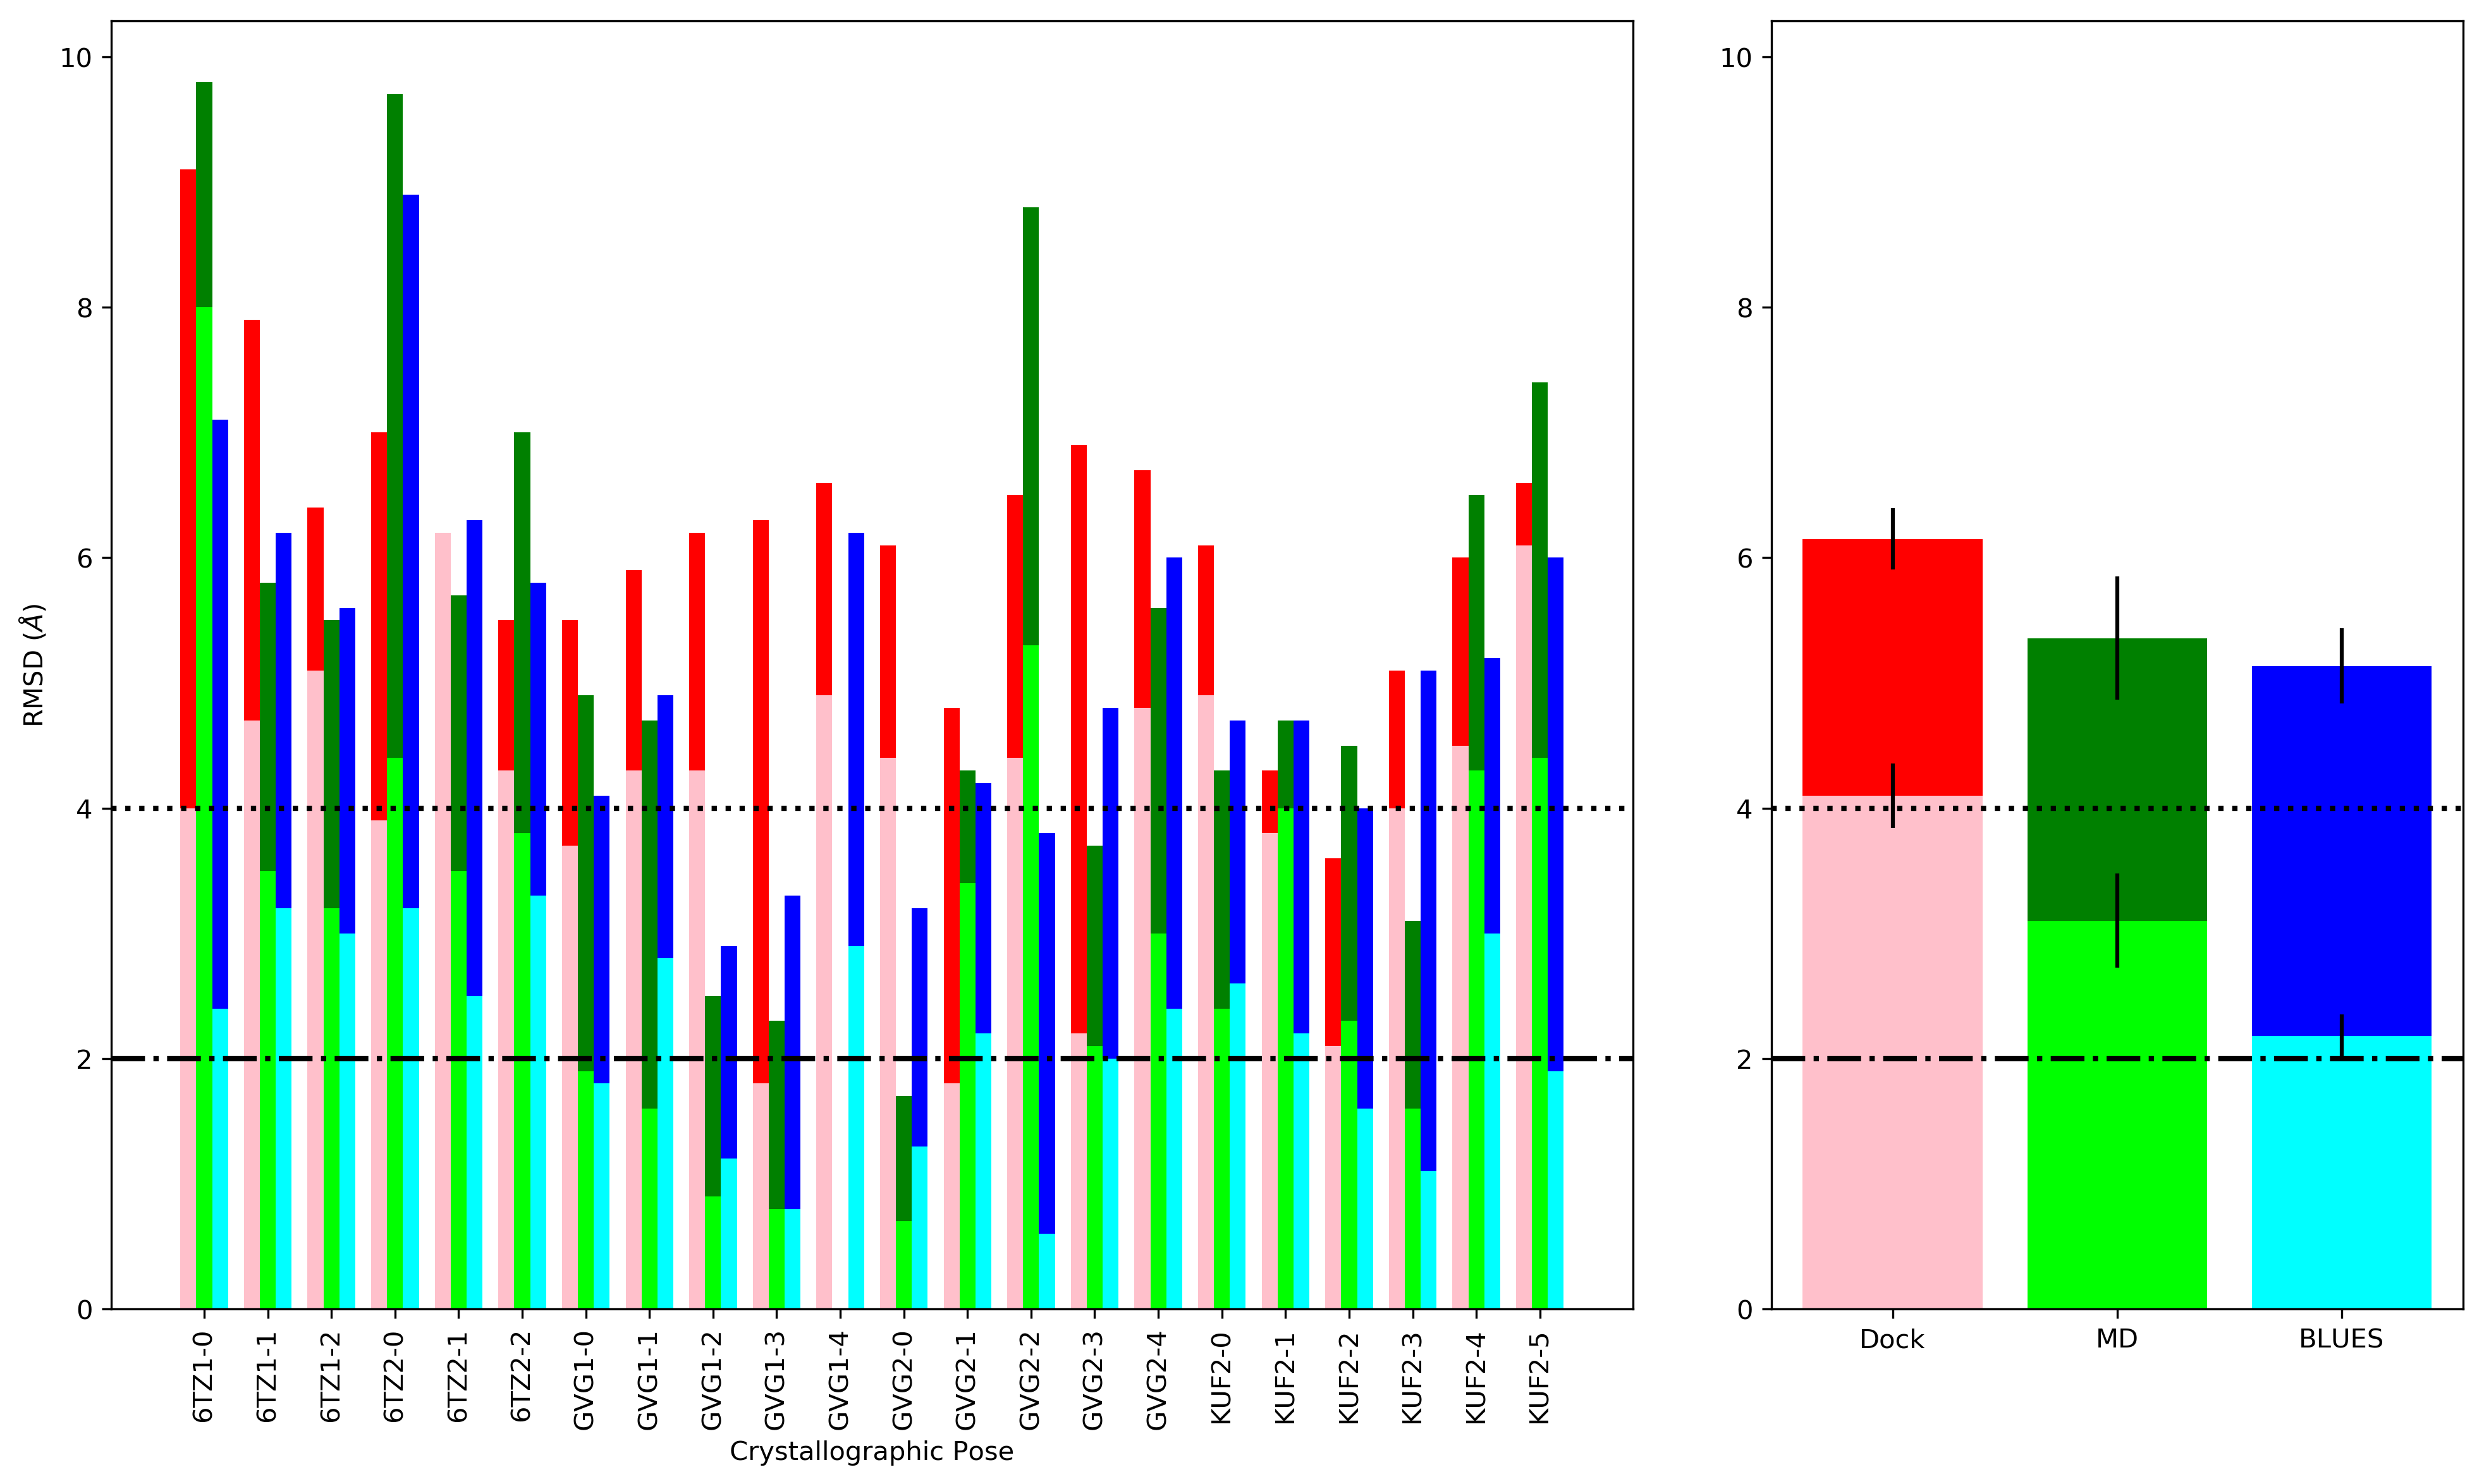
\includegraphics{chapter6/Figures/multibm.png}
    \caption[Multiple Binding Mode RMSDs]{Left: Calculated RMSDs (minimum/average) relative to the crystallographic ligand binding mode and binding modes from docking (pink/red), MD (lime/green), and BLUES (cyan/blue) simulations for ligands with a single binding mode. Successful prediction in binding mode is judged to be less than or equal to 2 {\AA} (black dashed horizontal line). Right: Averaged RMSDs for each method: docking, MD, and BLUES for ligands with a single binding mode. Considering the minimum RMSD averaged across ligands with a single binding mode, BLUES can make predictions with 2{\AA} to the true binding mode.}
    \label{fig:multibm}
\end{figure}

Molecules with multiple binding modes were 6TZ(1/2), GVG(1/2), and KUF which had 3, 5, and 6 crystallographic binding modes, respectively.
We note that simulations of 6TZ(1/2) or GVG(1/2) are simply the same molecules but different tautomers.
We consider these separately as we did not know prior, which were the correct tautomers to be simulating.
We compare binding modes sampled in simulations of 6TZ(1/2) and GVG(1/2) to the same crystallographic structures, respectively.
The RMSD for each molecule to each crystallographic structure is denoted as XXXX-#; for example, 6TZ1-(0,1,2) is the comparison from the simulations if 6TZ1 against the 3 crystallographic binding structures.

6TZ1 had 3 crystallographic binding modes with minimum RMSDs of 4.0, 4.7, and 5.1 from docking; 8.0, 3.5, and 3.2 from MD; and 2.4, 3.2, and 3.0 from BLUES.
The average RMSDs were reported to be 9.1, 7.9, and 6.4 from docking; 9.8, 5.8, and 5.5 from MD; and 7.1, 6.2, and 5.6 from BLUES.
Likewise for 6TZ2, the minimum RMSDs were 3.9, 6.2, and 4.3 from docking; 4.4, 3.5 and 3.8 from MD; and 3.2, 2.5, and 3.3 from BLUES.
The average RMSDS were reported to be 7.0, 6.2, and 5.5 from docking; 9.7, 5.7, and 7.0 from MD; and 8.9, 6.3, and 5.8 from BLUES.
There were no successful predictions for 6TZ(1/2) using either docking, MD or BLUES when considering either the minimum or average RMSDs.
In the cases of 6TZ(1/2), using MD and BLUES generally resulted in predictions which were close (within 4{\AA} of the crystallographic structure, with docking only coming close in 2 out of the 6 cases (represented in 6TZ1/2-0).
From this data, we cannot definitively say which tautomer for 6TZ was the correct one to be simulating.

GVG1 and GVG2 had 5 crystallographic binding modes to compare our predictions to, which are denoted with GVG(1/2)-(0,1,2,3,4).
Here, we note that MD simulations of GVG1 did not sample enough metastable states to have a prediction for each crystallographic binding mode--missing 1 prediction for GVG1-4.
The minimum RMSDs to GVG1 were 3.7, 4.3, 4.3, 1.8, and 4.9 for docking; 1.9, 1.6, 0.9, 0.8, and NF (NF-Not Found) for MD; and 1.8, 2.8, 1.2, 0.8, and 2.9 for BLUES.
The average RMSDs to GVG1 were 5.5, 5.9, 6.2, 6.3, and 6.6 from docking; 4.9, 4.7, 2.5, 2.3, and NF for MD; and 4.1, 4.9, 2.9, 3.3, and 6.2 for BLUES.
When considering the average RMSD, there were no successful predictions of the crystallographic binding mode with any method for GVG1.
If we consider the minimum RMSD for GVG1, we see successful predictions using docking in GVG1-3 (1/5), using MD in GVG1-0,1,2,3 (4/5) and using BLUES in GVG1-0,2,3 (3/5).

The minimum RMSDS to GVG2 were 4.4, 1.8, 4.4, 2.2, and 4.8 from docking; 0.7, 3.4, 5.3, 2.1, and 3.0 from MD; and 1.3, 2.2, 0.6, 2.0, and 2.4 from BLUES.
The average RMDs to GVG2 were 6.1, 4.8, 6.5, 6.9, and 6.7 from docking; 1.7, 4.3, 8.8, 3.7, and 5.6 from MD; and 3.2, 4.2, 3.8, 4.8, and 6.0 from BLUES.
Based on the average RMSDs for GVG2, we see 1/5 successful case (GVG2-0) with MD but not for any other method.
Considering the minimum RMSDs, we see successes in 1/5 cases for docking (GVG2-1) and MD (GVG2-0), while with BLUES we see successes in 3/5 cases (GVG2-0,2,3).
In comparing the results of GVG1 versus GVG2, we believe the data suggests that simulations of GVG1 was the correct tautomer to be simulating.

Finally, KUF2 had 6 crystallographic binding modes to compare our predictions to.
The minimum RMSDs were 4.9, 3.8, 2.1, 4.0, 4.5, and 6.1 from docking; 2.4, 4.0, 2.3, 1.6, 4.3 and 4.4 from MD; and 2.6, 2.2, 1.6, 1.1, 3.0, and 1.9 from BLUES.
The average RMSDs were 6.1, 4.3, 3.6, 5.1, 6.0, and 6.6 from docking; 4.3, 4.7, 4.5, 3.1, 6.5, and 7.4 from MD; and 4.7, 4.7, 4.0, 5.1, 5.2, and 6.0 from BLUES.
There we no successes when considering the average RMSD for KUF2.
For KUF2, successes were seen in 3/6 cases when considering the minimum RMSD using BLUES simulations (KUF2-2,3,5) and in 1/6 cases using MD (KUF2-3).

For this subset of ligands which multiple binding modes, the collective minimum RMSD was $4.1 \pm 0.3$, $3.1 \pm 0.4$, and $2.2 \pm 0.2$ from docking, MD, and BLUES, respectively.
The collective average RMSD was $6.1 \pm 0.2$, $5.4 \pm 0.5$, and $5.1 \pm 0.3$ from docking, MD and BLUES, respectively.
When considering the minimum RMSD from docking and MD, these methods can make predictions which are close (within 4{\AA}) to the crystallographic structures, if there are multiple binding modes.
With BLUES, one may be able to make predictions which are within 2 {\AA} as we observe sampling which is much closer to the true binding modes even if there are several.

\section{Discussion}
\subsection{Single Binding Mode: Both MD and BLUES eventually find 1 crystallographic binding mode}

\begin{figure}[!tbp]
  \centering
  \subfloat{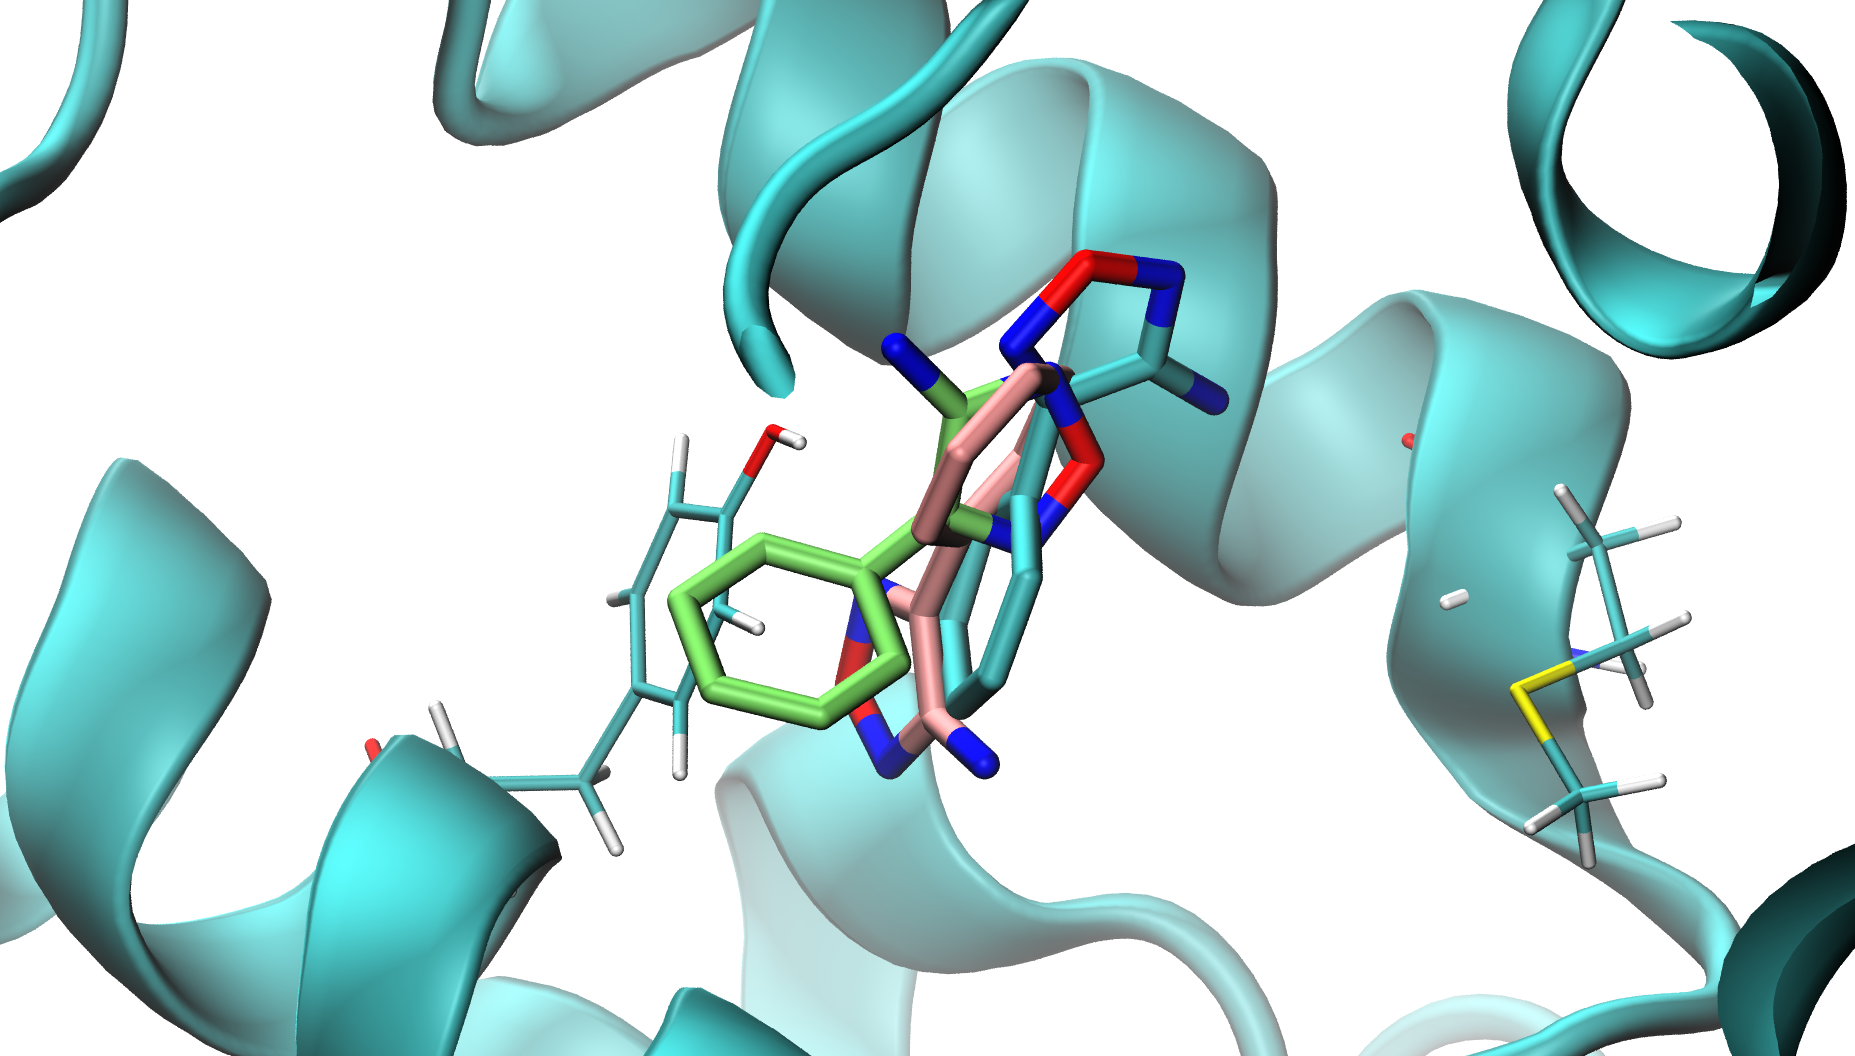
\includegraphics[width=0.5\textwidth]{chapter6/Figures/JF6_1-poses.png}\label{fig:JF6-poses}}
  \hfill
  \subfloat{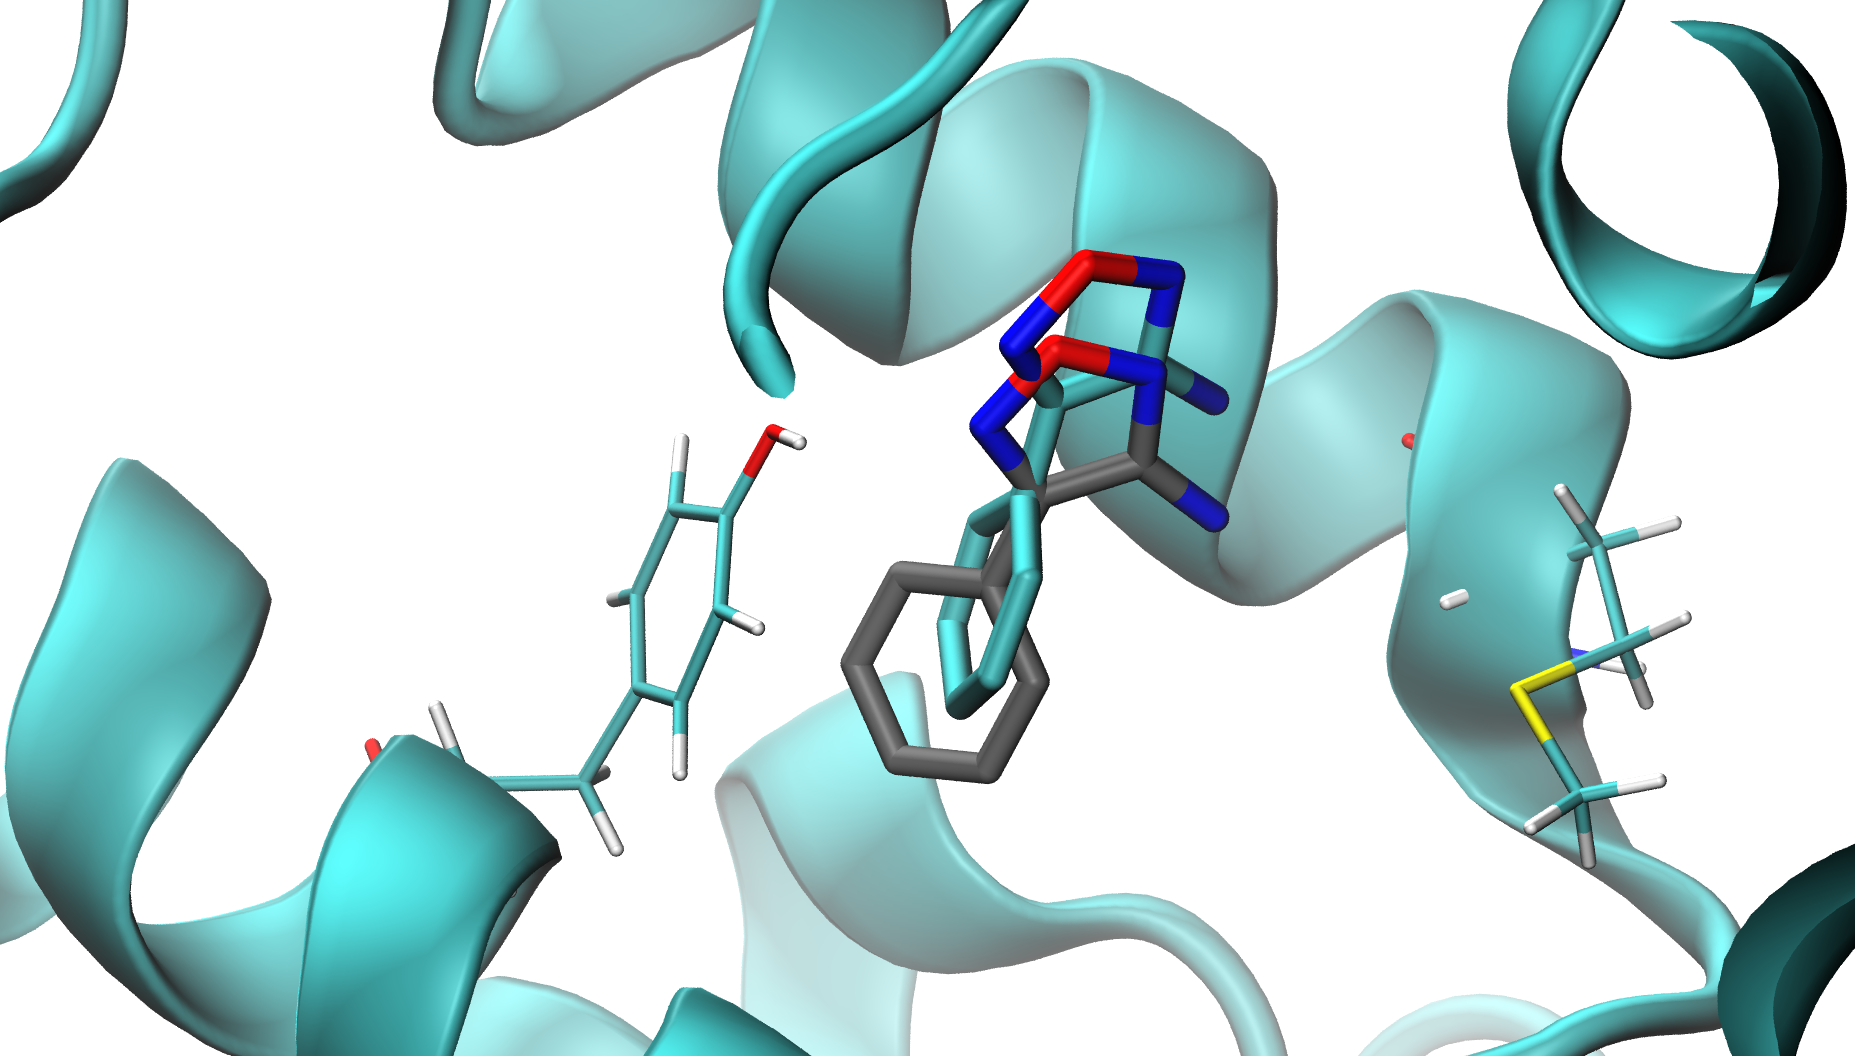
\includegraphics[width=0.5\textwidth]{chapter6/Figures/JF6_1-xtal.png}\label{fig:JF6-xtal}}
  \caption[JF6 docked poses and crystal structure]{Left: Docked pose of JF6 (pink) and simulation frames from MD (lime) and BLUES (cyan) which minimizes the RMSD to the crystallographic structure. This binding mode for JF6 was located in the left sub-cavity. The minimum RMSDs were 4.5, 3.6, and 1.5 for docking, MD, and BLUES, respectively. Right: BLUES (cyan) simulation frame with the crystallographic binding mode (gray) for molecule JF6. Nearby residues TYR117(?) and MET243(?) are shown.}
\end{figure}

When considering the minimum RMSDs, for cases with a single crystallographic binding mode, we see that both MD and BLUES are within 2 {\AA} of the crystallographic binding mode.
On the other hand, docking will--at best--make predictions which are close (within 4{\AA}) to the crystallographic binding mode.
We note that here, we simulate 1 microsecond of MD and 600ns of BLUES for each remaining pose after our MDS-RMSD filter, so our relative success with BLUES indicates that BLUES may find the crystallographic binding mode much faster than traditional MD.

We will first discuss our observations from JF6, where BLUES is able to find the crystallographic binding mode while MD did not, as this case helps illustrate the relative advantages of the BLUES approach.
In this case, the closest docked pose for JF6 was 4.5 {\AA} away from the crystallographic binding mode (Fig. \ref{fig:JF6-poses}), where the molecule is completely flipped in the opposite orientation from the crystallographic binding mode.
Following that, we will present our findings from 8NY where both BLUES and MD successfully identify the crystallographic binding mode (notably faster with MD over BLUES), but we will show that BLUES facilitates sampling of more binding modes than MD--even if they are not found by crystallography.

\begin{figure}
    \centering
    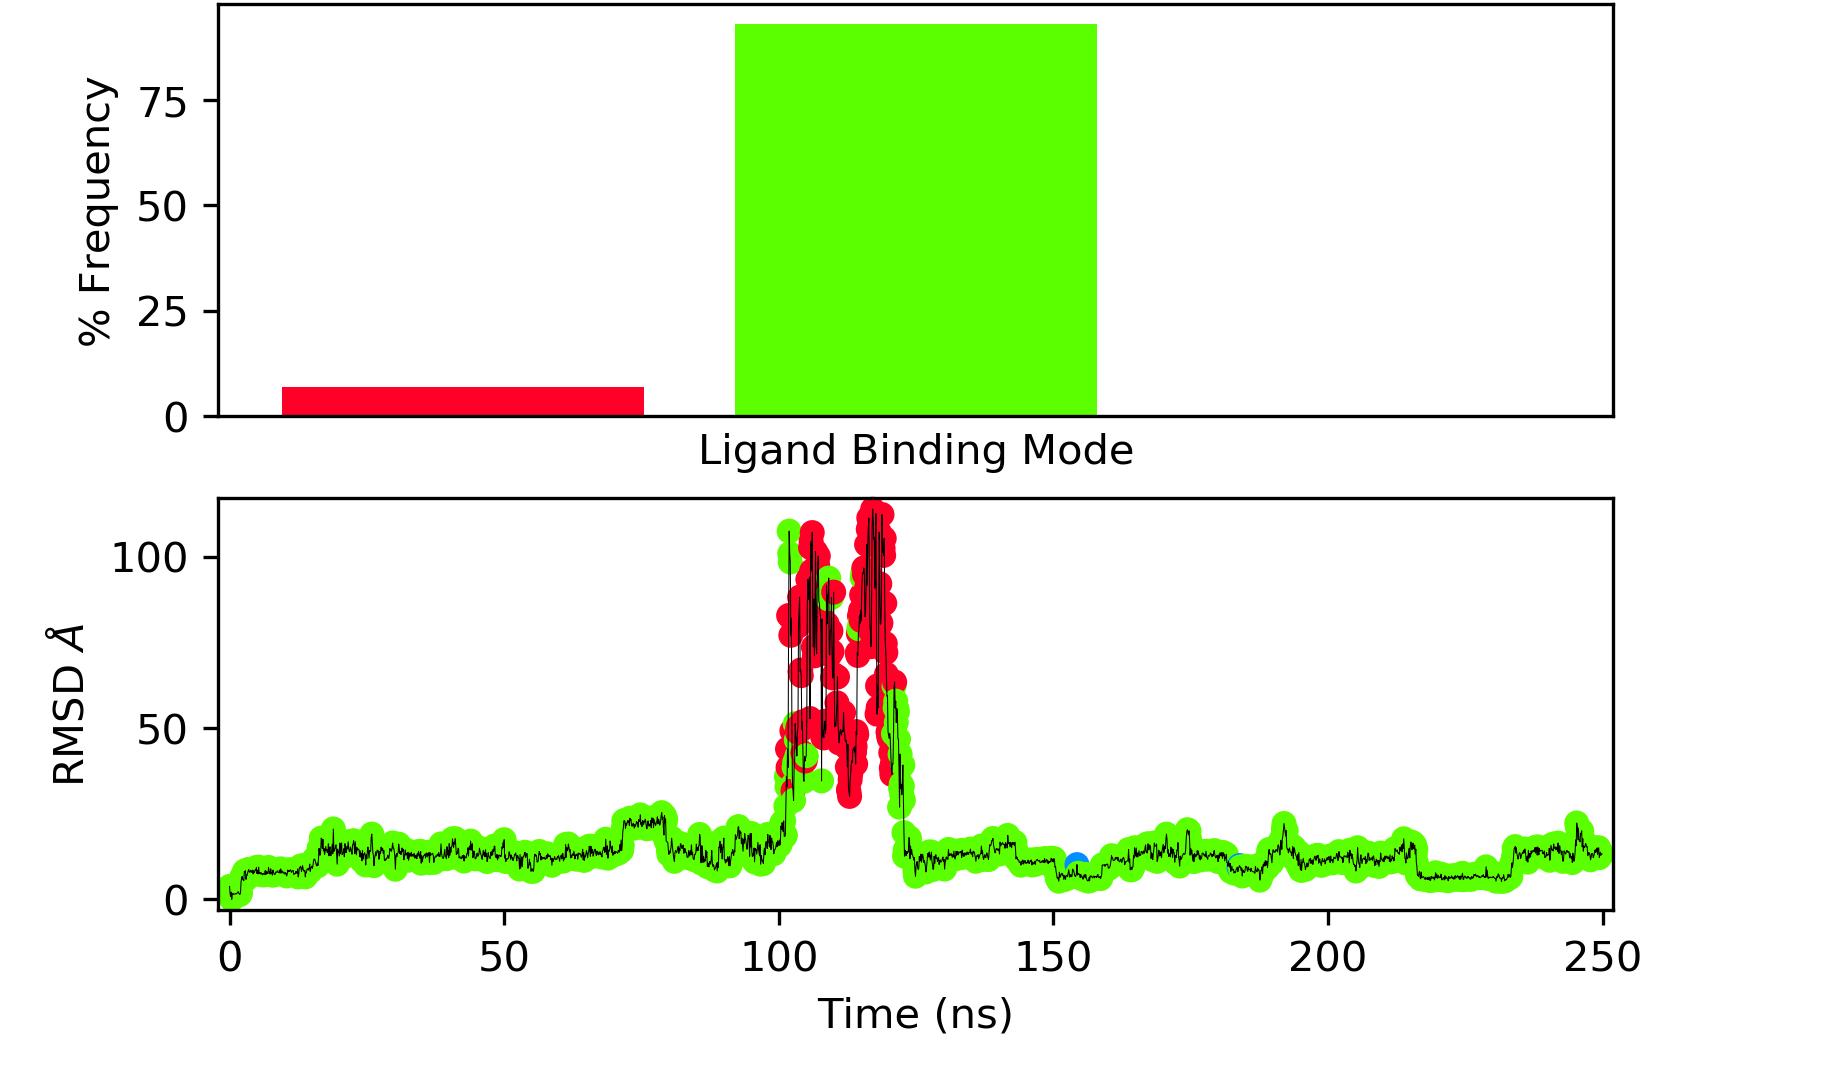
\includegraphics{chapter6/Figures/JF6_c4-prod00.png}
    \caption[JF6 MD Populations]{Top: 250ns MD populations (\% simulation time) of 2 (red/green) binding modes sampled for ligand JF6. Bottom: RMSD of ligand JF6 relative to starting positions over time. Each time point is colored according to the binding mode the ligand is in. We note that the red samples correspond to an unbound state. Thus, this shows that with MD we only sample 1 binding mode (green).}
    \label{fig:JF6_c4-md}
\end{figure}

In Figure \ref{fig:JF6_c4-md}, we show the first 250ns from MD for JF6, where we see sampling of primarily only a single binding mode (green).
Shortly after 100ns, JF6 was observed to unbind from the binding site (indicated in red) and then return to the binding site, where it samples the same primary binding mode (green).
The primary binding mode sampled during MD was 9.1 {\AA} away from the crystallographic binding (on average) and at best was 3.6 {\AA} away (Fig. \ref{fig:JF6-poses}).
For the remainder of the 1 microsecond simulation, JF6 remains trapped in the green binding mode and never transitions out in order to find the crystallographic binding mode or at the very least, another binding mode which is close to it.

\begin{figure}
    \centering
    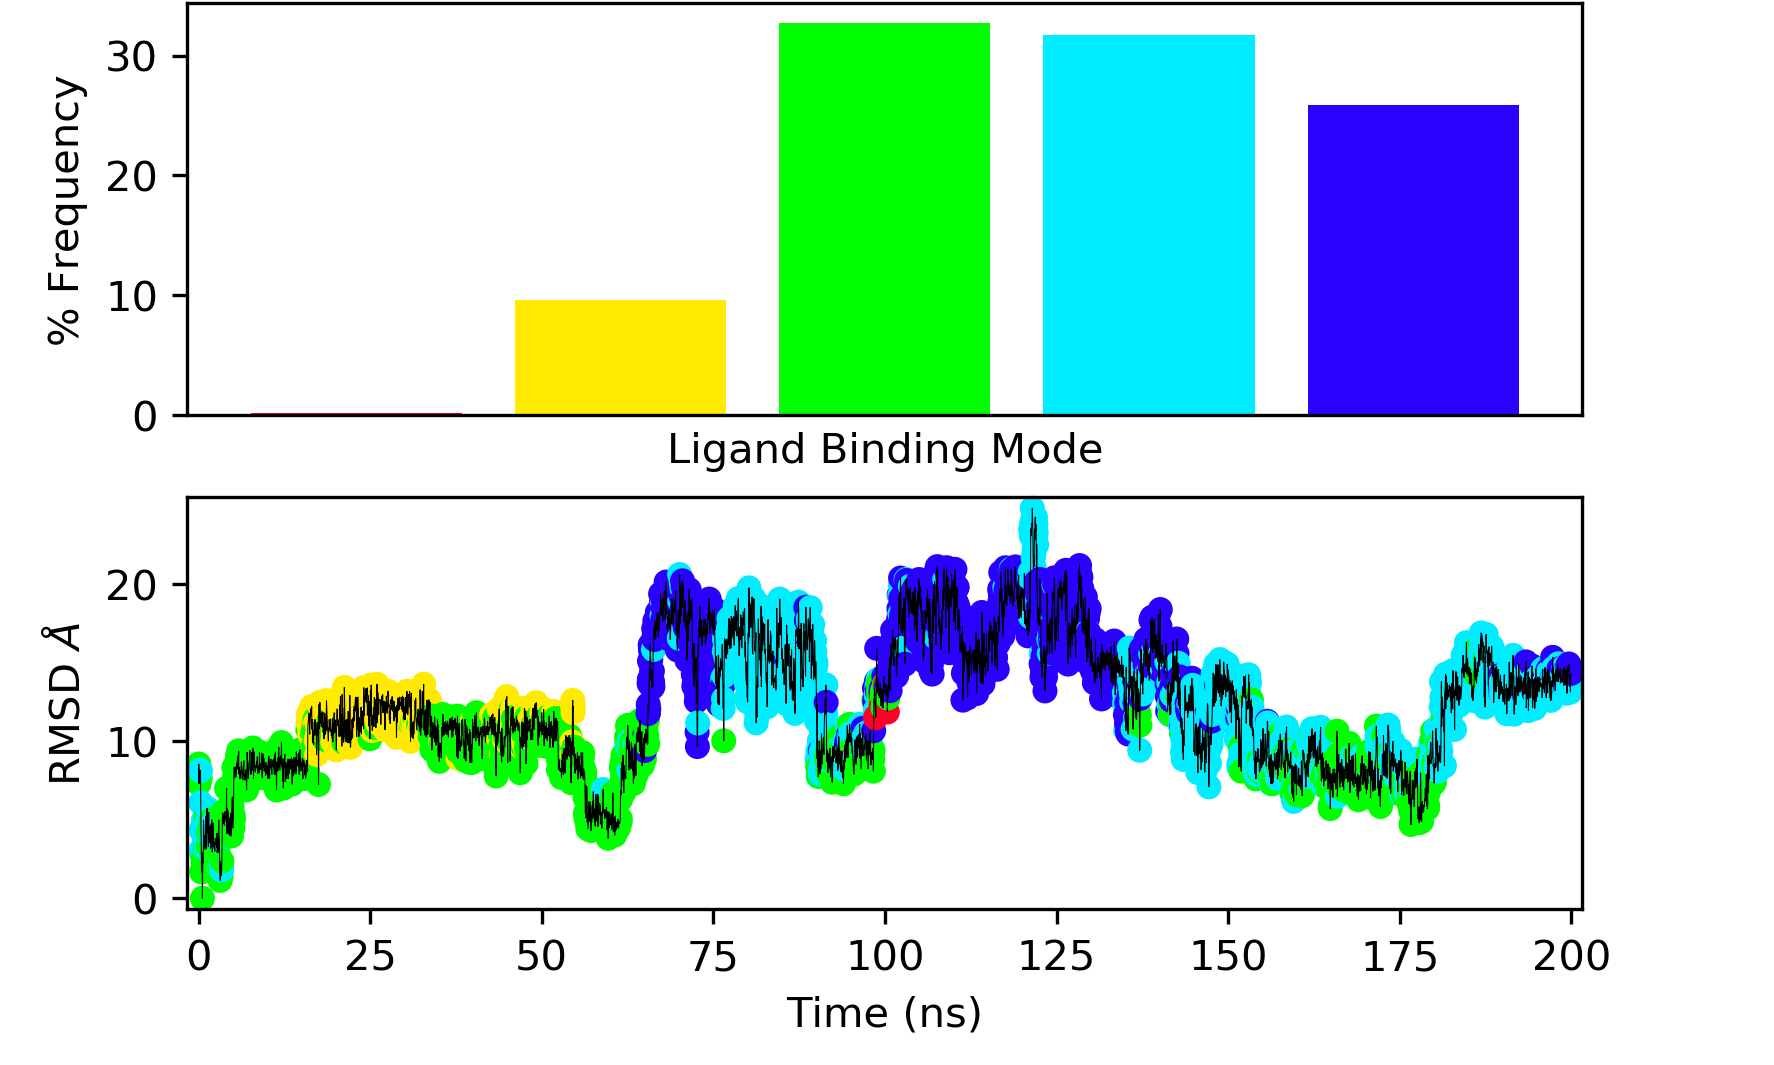
\includegraphics{chapter6/Figures/JF6_c4-14607404.png}
    \caption[JF6 BLUES Populations]{Top: 200ns BLUES populations (\% simulation time) of 5 (red, yellow, green, cyan, blue) binding modes sampled for ligand JF6. Bottom: RMSD of ligand JF6 relative to starting positions over time. Each time point is colored according to the binding mode the ligand is in. This shows BLUES can sample far more binding modes than MD in a shorter timeframe. Note: we see no red bar due to extremely low sampling during the simulation.}
    \label{fig:JF6_c4-blues}
\end{figure}

In contrast, we see from Figure \ref{fig:JF6_c4-blues} a 200ns BLUES simulation, where we observe sampling of 5 different binding modes, with the dominant binding mode represented in green.
Most notably, with BLUES, we see fairly good sampling as we observe several transitions in and out of the dominant binding mode (green).
This is indicative that BLUES does indeed accelerate sampling of ligand binding modes for this particular fragment.
Here, the dominant (green) binding mode had an average RMSD of 6.6 {\AA} but at best sampled 1.5 {\AA} away (Fig. \ref{fig:JF6-poses}) from the crystallographic binding mode.
Although the average RMSD was much higher than the 2 {\AA} cutoff in this case, we believe this could be due to the fact that JF6 doesn't reside in the green binding mode for a very a long period of time, which would lower our averaged RMSD calculation.
Instead, we see many transitions into the green binding mode for brief periods of time, where at some point the ligand was very close to the crystallographic binding mode.
Regardless, this shows that our BLUES approach does facilitate sampling of more than just a single binding mode in a shorter time span; which is in stark contrast to what we observed in our 1 microsecond MD simulation.

\begin{figure}
    \centering
    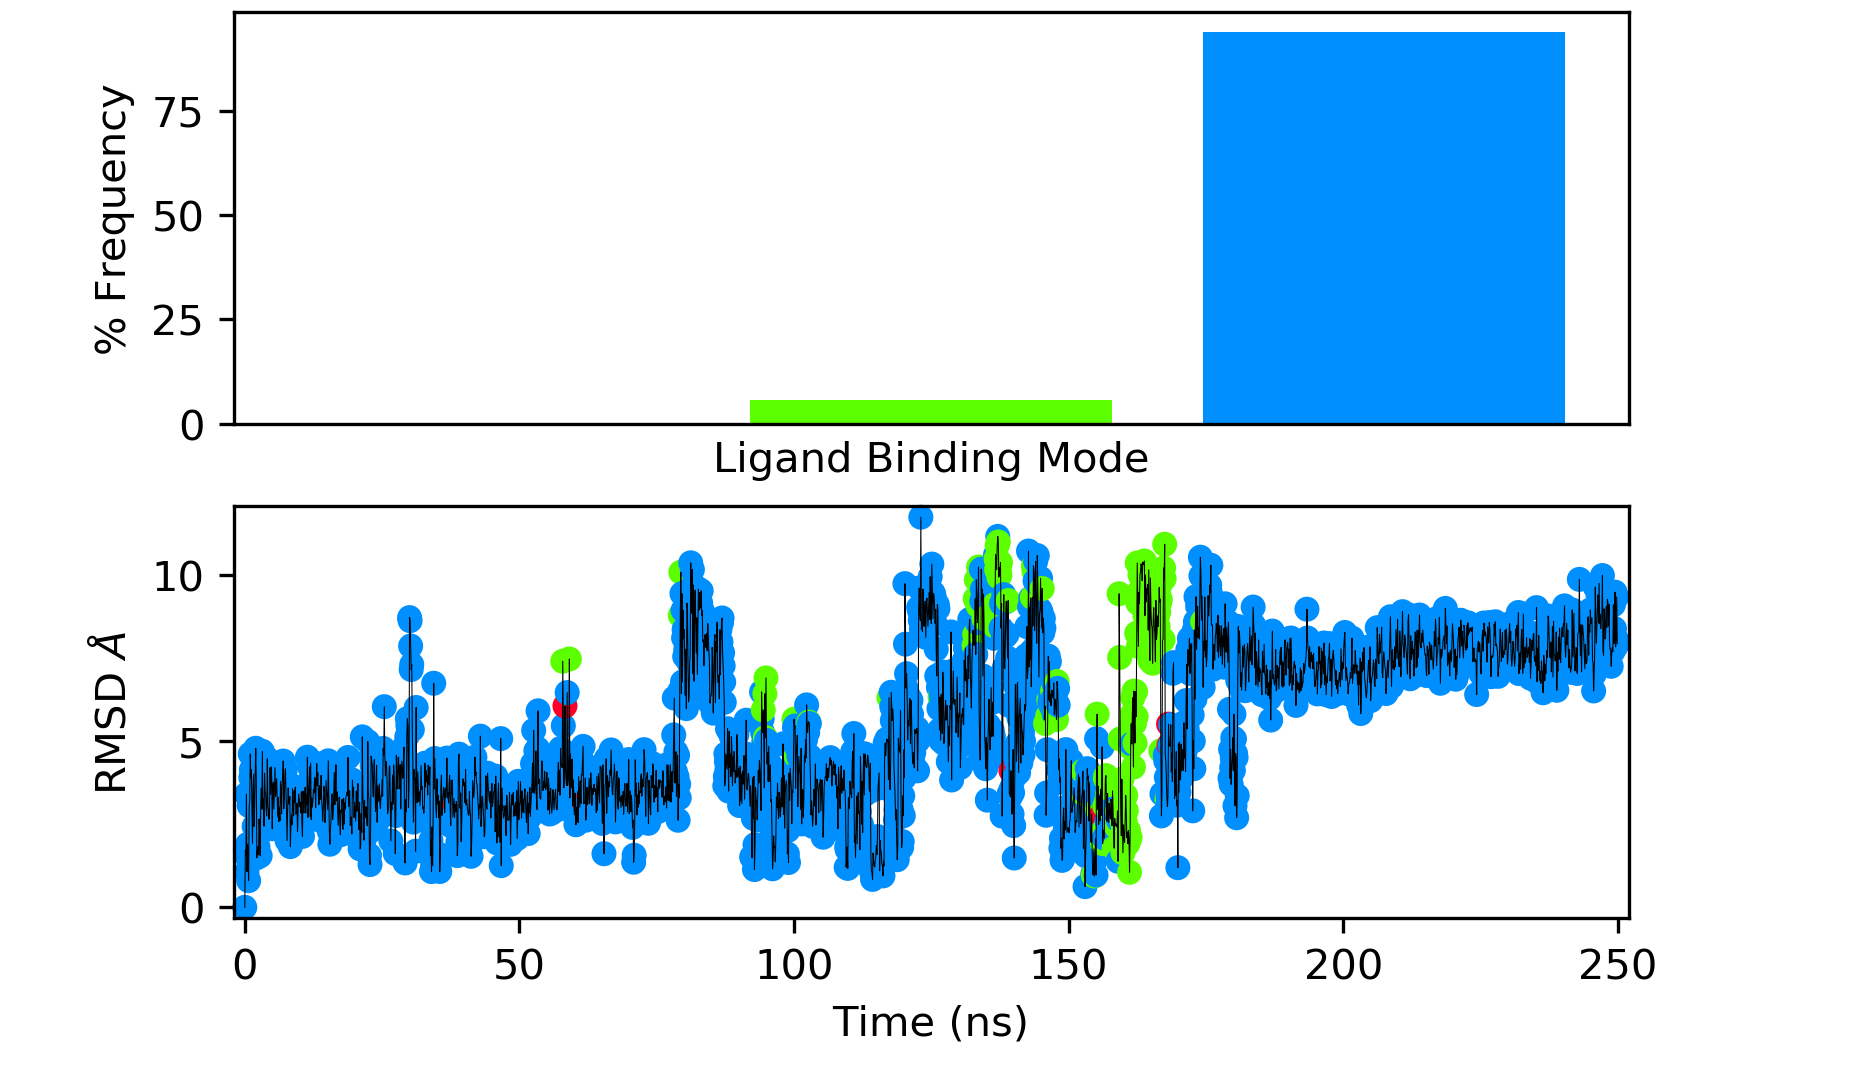
\includegraphics{chapter6/Figures/8NY_c0-prod00.png}
    \caption[8NY MD populations]{Top: 250ns MD populations (\% simulation time) of 3 (red, green, blue) binding modes sampled for ligand 8NY. Bottom: RMSD of ligand 8NY relative to starting positions over time. Each time point is colored according to the binding mode the ligand is in.}
    \label{fig:8NY_c0-md}
\end{figure}

In Figure \ref{fig:8NY_c0-md}, we show the first 250ns from MD for 8NY, where we see sampling of the dominant binding mode (blue) and very brief sampling of 2 other binding modes (red/green)--albeit not stably.
Here, the blue binding mode was calculated to be 1.8 {\AA} away from the crystallographic binding mode (on average), demonstrating MD can indeed identify the crystallographic binding mode within a short time frame.
Despite an accurate prediction, we highlight that we primarily only see stable sampling of the blue binding mode using MD rather than observing sampling of alternative binding modes.

\begin{figure}
    \centering
    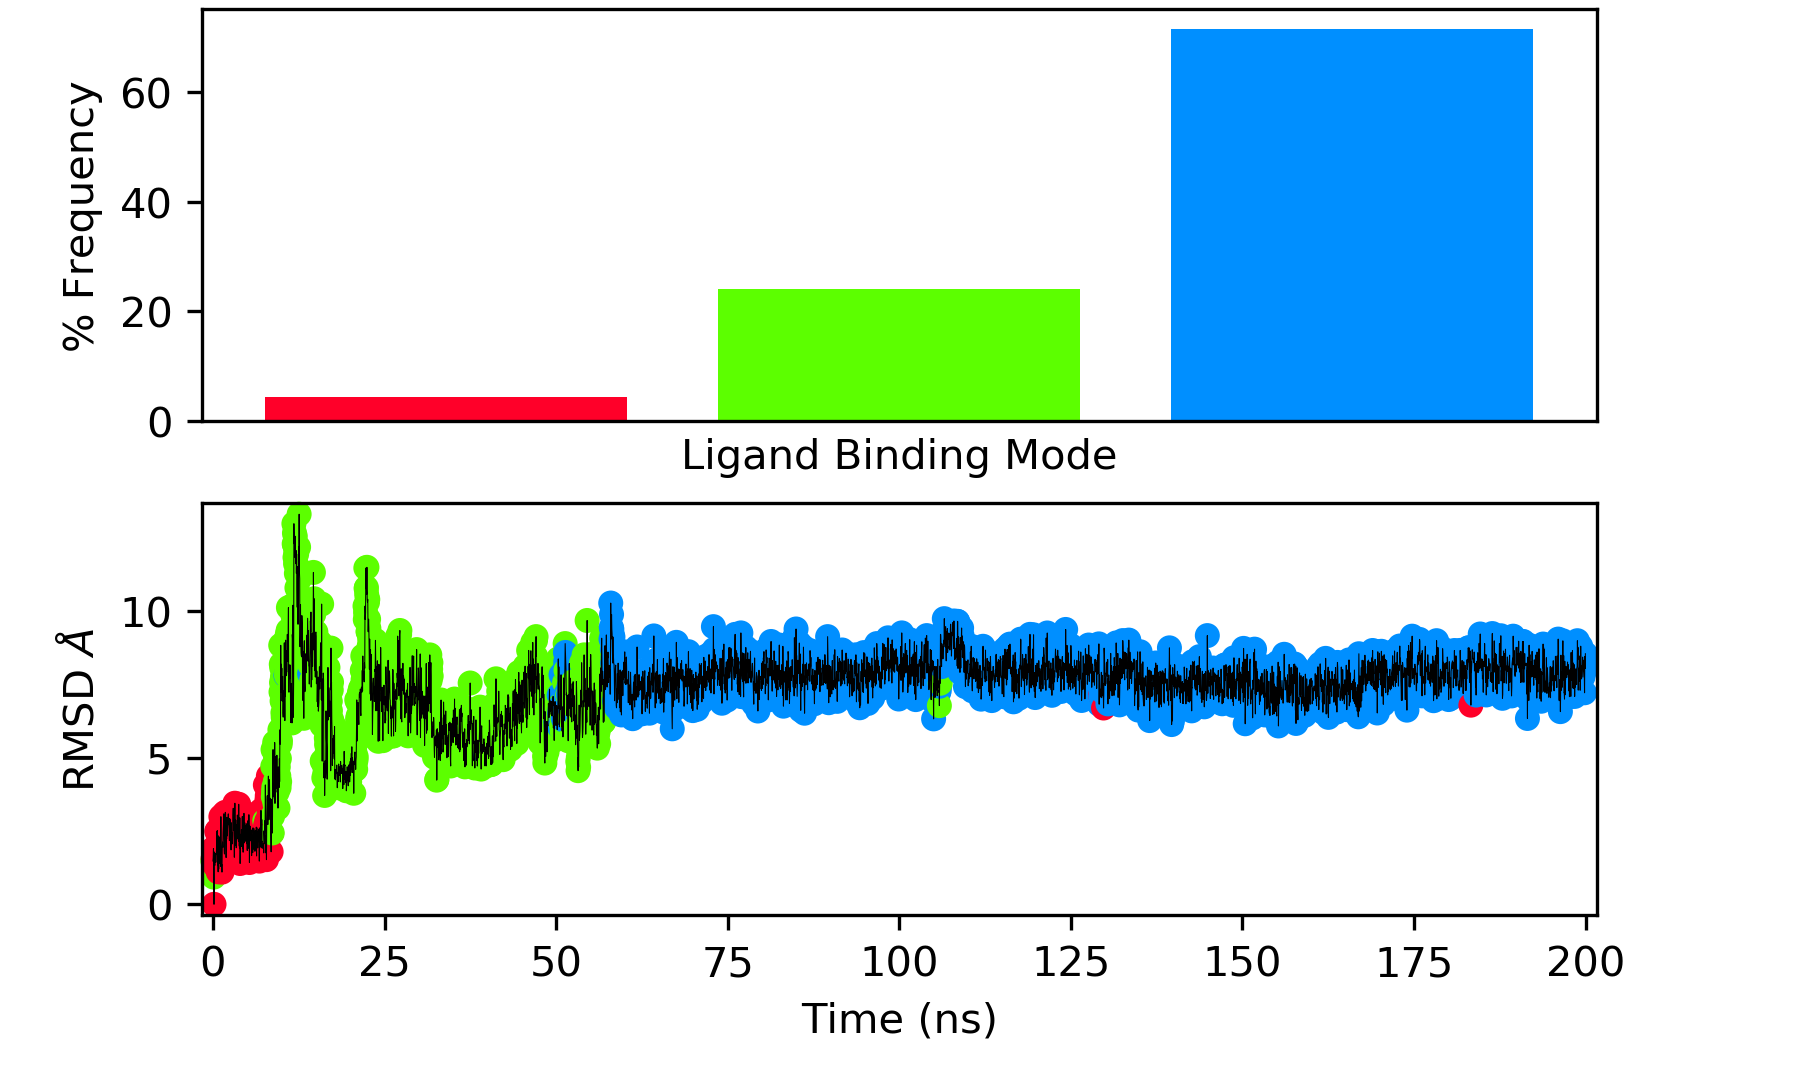
\includegraphics{chapter6/Figures/8NY_c0-14708877.png}
    \caption{Top: 200ns BLUES populations (\% simulation time) of 3 (red, green, blue) binding modes sampled for ligand 8NY. Bottom: RMSD of ligand 8NY relative to starting positions over time. Each time point is colored according to the binding mode the ligand is in.}
    \label{fig:8NY_c0-blues}
\end{figure}

From Figure \ref{fig:8NY_c0-blues}, we see better sampling of ligand binding modes with BLUES.
Here, we observe fairly stable sampling of 3 different binding modes in a shorter time frame than MD (200ns).
Here, BLUES begins in the red binding mode before transitioning into the green binding mode after 10ns, where it remains in until we observe another transition at 60ns into the blue binding mode.
This blue binding mode observed after 60ns ends up as the most populated binding mode over the course of the simulation and was calculated to be 1.5 {\AA} away from the crystallographic binding mode.
In this case, we note that BLUES did take longer to find the crystallographic binding mode than MD, but we see better sampling of alternative ligand binding modes which are not seen in the crystallographic structure.
We hypothesize that these alternative binding modes found via BLUES represent metastable states in which the fragment may bind in, before settling on the primary binding mode represented in the crystallographic structure.

For all ligand with a single binding mode, when we consider the averaged RMSDs, we find that both MD and BLUES are equally able to make close predictions (within 4 {\AA}) to the crystallographic binding mode, when there is only 1 binding mode to identify (Right: Figure \ref{fig:singlebm}).
On average, for this subset of fragments, MD identified the crystallographic binding mode in 1/7 cases and in 2/7 cases using BLUES.
If we consider the minimum RMSD--representing having sampled near the true binding mode--we find that MD and BLUES also both are able to identify a single crystallographic binding mode within 2 {\AA} (Right: Figure \ref{fig:singlebm}).
Here, considering the minimum RMSDs to the crystallographic structure, MD identified 5/7 and BLUES identified 7/7 cases.

While both BLUES and MD are able to sample and find the crystallographic binding mode, BLUES seems to facilitate sampling of alternative ligand binding modes rather than remaining trapped in 1-2 binding modes like with MD.
In some cases (like with JF6) BLUES may be able to find the crystallographic binding mode much faster than MD and in other cases it may not (like with 8NY).
In general, with BLUES, we observe not only more sampling of other ligand binding modes (8NY), but we also observe more transitions between binding modes (JF6), which gives us better estimates of the populations for these small and rigid fragments.
Here, we highlight that with accelerated sampling from BLUES, one may be able to gain more structural insight on alternative ways the ligand may bind in the binding site, which are not be captured in the crystallographic structure.

\subsection{Multiple Binding Modes: Sampling binding mode transitions leads to more accurate predictions}
In our observations from the single binding mode cases, we highlighted the importance of sampling more ligand binding modes and transitions between them.
That is, when we observed more binding mode transitions (particularly with BLUES), we saw that the minimum RMSD (and in some cases the average) was much closer to the crystallographic binding mode.
For cases with multiple binding modes, we believe sampling of more binding mode transitions during our simulations is even more critical as there are more crystallographic binding modes to be identified.

\begin{figure}
    \centering
    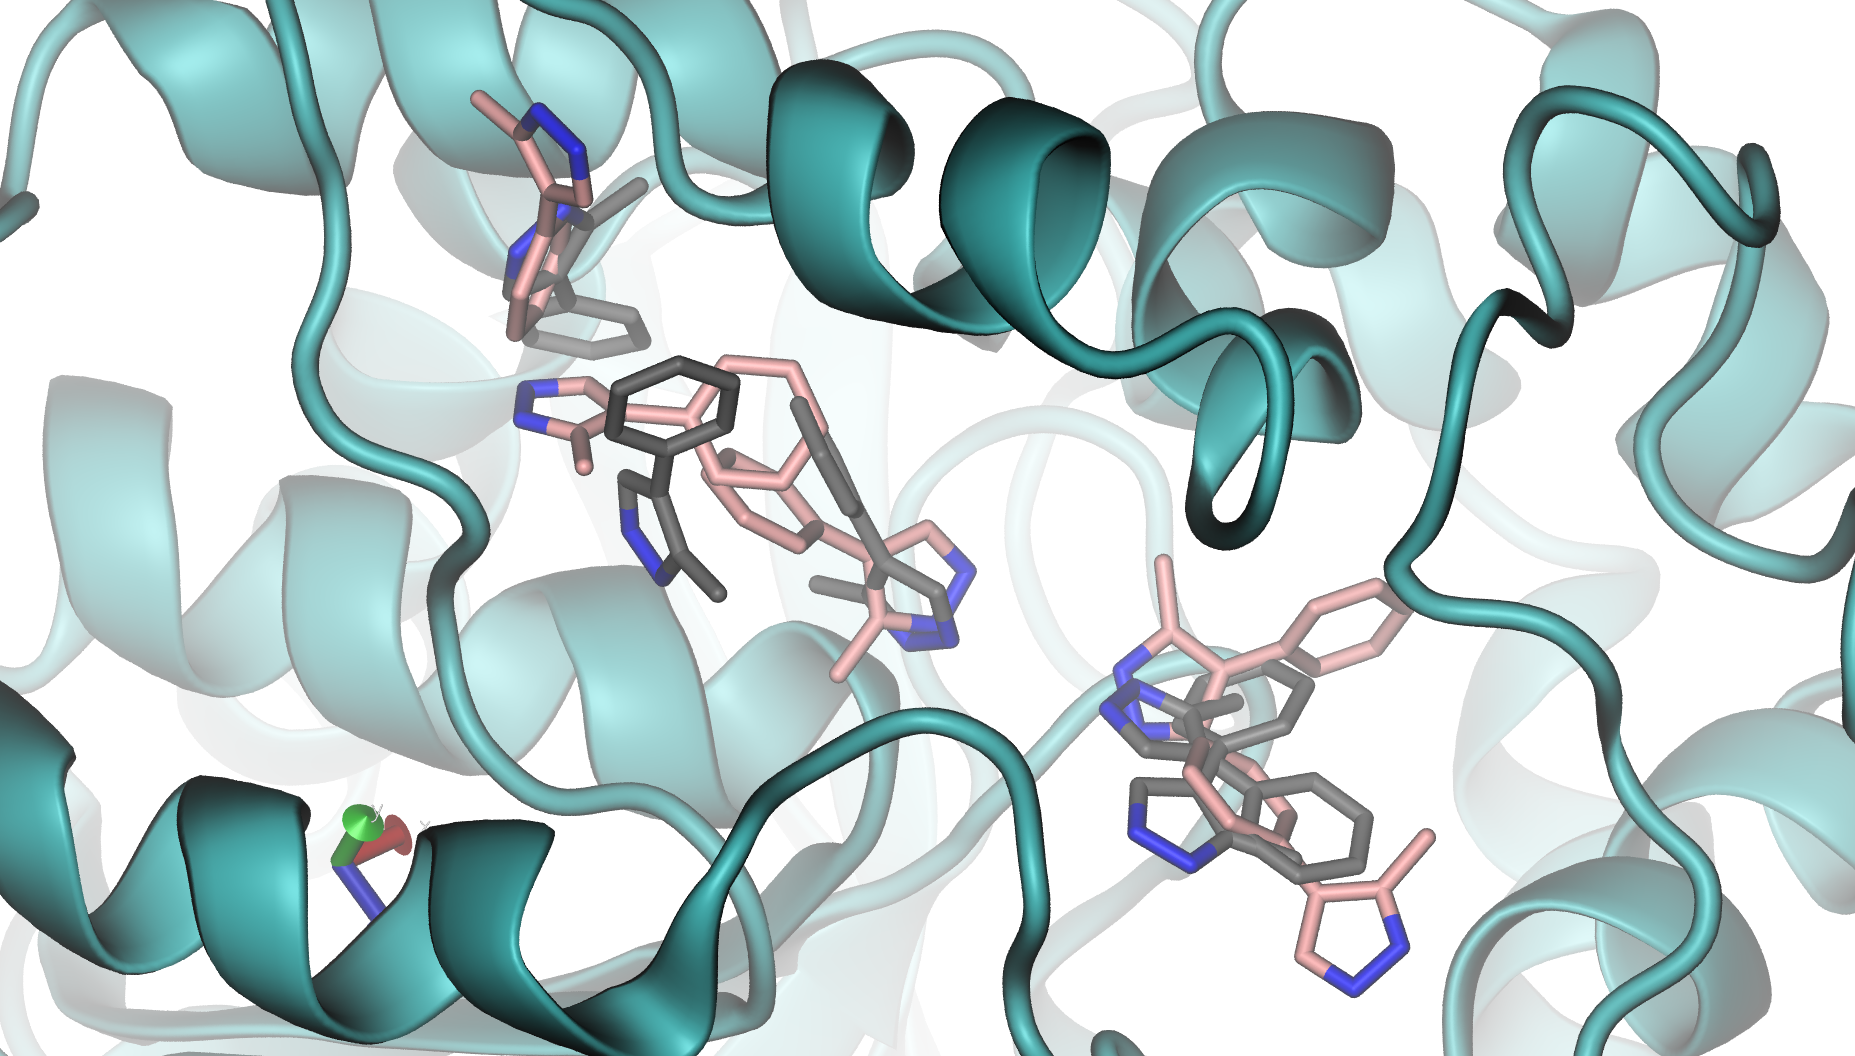
\includegraphics{chapter6/Figures/GVG_1-poses.png}
    \caption[GVG1 docked poses]{5 crystallographic binding modes (gray) for molecule GVG1 overlaid with the starting poses from docking (pink).}
    \label{fig:GVG1-poses}
\end{figure}

Here, we will present our observations from MD and BLUES simulations of GVG1, where we surprisingly observed more binding mode transitions using MD in the right sub-cavity.
This led to more accurate predictions (when considering the minimum RMSD) for MD over BLUES; where with BLUES, we saw sampling of only 1 binding mode and thus failed to identify the secondary binding mode in the right sub-cavity.
This is an atypical case, where much like we have shown previously, BLUES facilitates sampling of more binding modes and transitions between them much more over traditional MD.

\begin{figure}
    \centering
    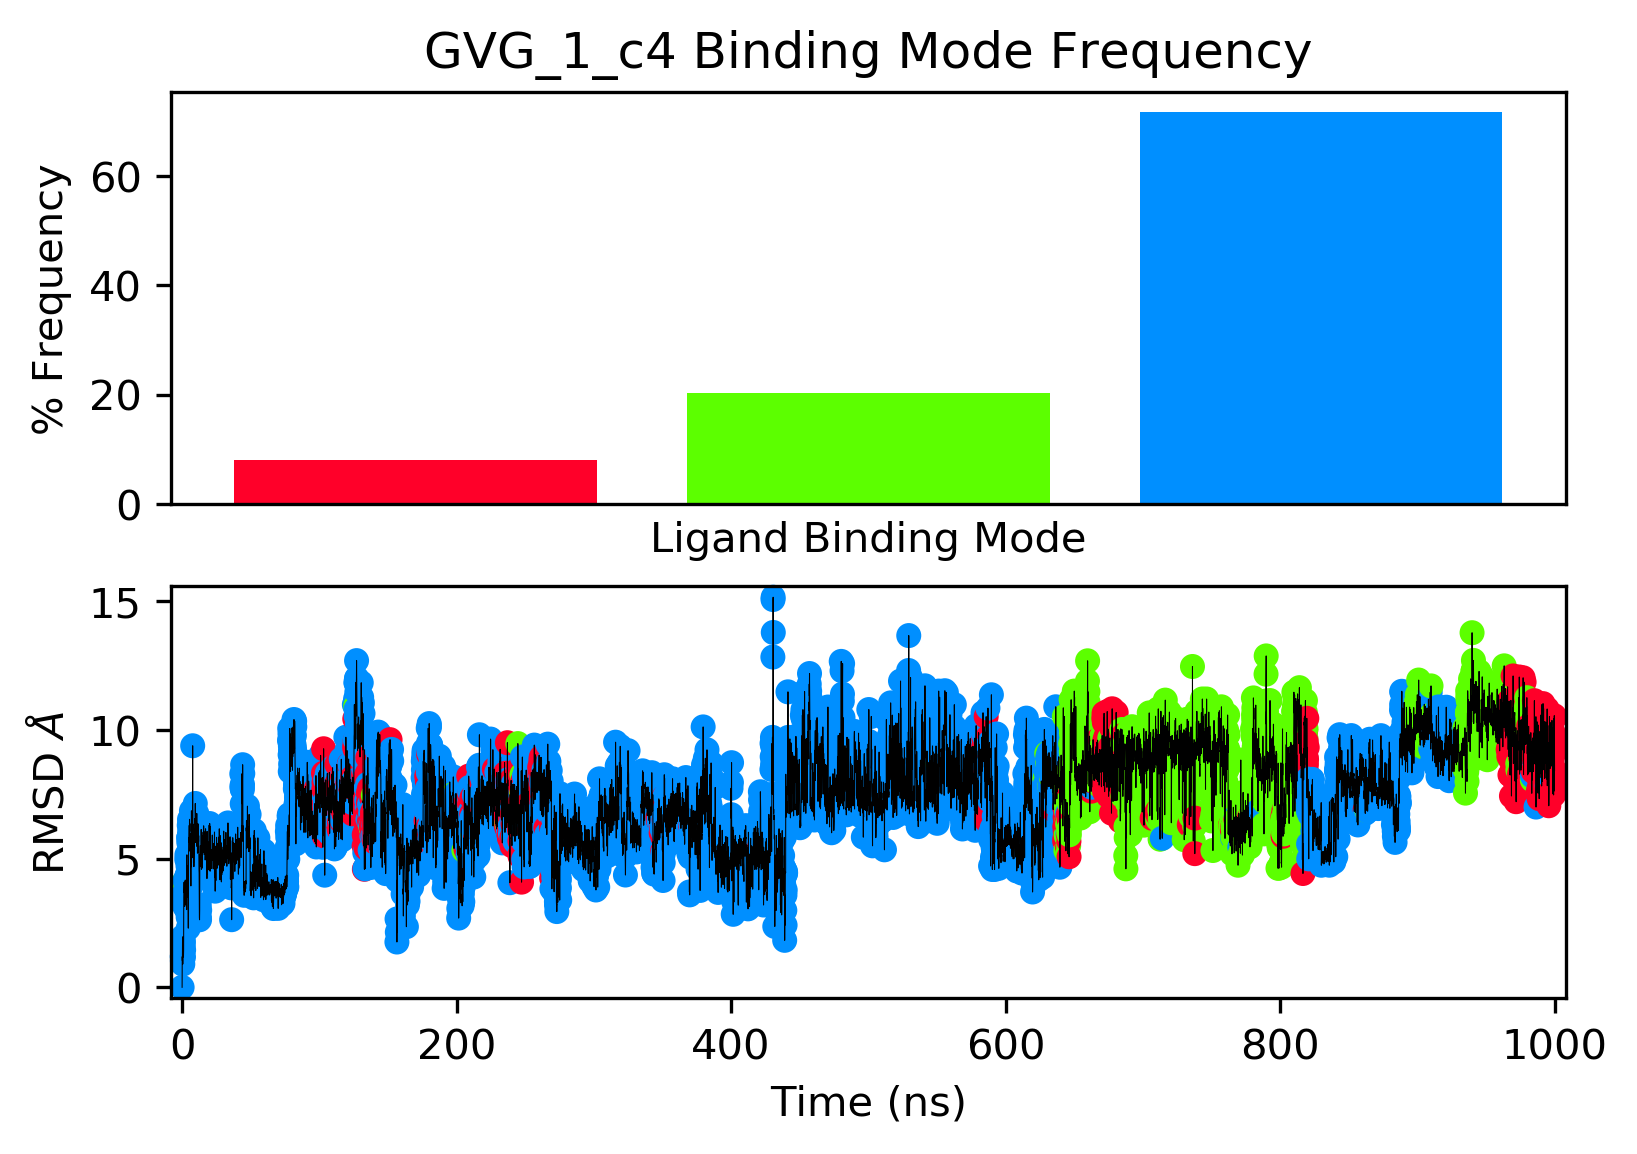
\includegraphics{chapter6/Figures/GVG_1_c4-md.png}
    \caption[GVG1 MD Populations]{Top: 1 microsecond MD populations (\% simulation time) of 3 (red, green, blue) binding modes sampled for ligand GVG1. Bottom: RMSD of ligand GVG1 relative to starting positions over time. Each time point is colored according to the binding mode the ligand is in.}
    \label{fig:GVG1_c4-md}
\end{figure}

For the case of GVG1, there were 2 binding modes to identify in the right sub-cavity and 3 in the left sub-cavity (Fig. \ref{fig:GVG1-poses}).
For the left sub-cavity, we started simulations from 3 different docked poses, where each of these independent simulation were able to find the 3 crystallographic binding modes.
In these simulations we did not observe transitions between the 3 binding modes in the left sub-cavity.
On the other hand, in the right sub-cavity (Fig. \ref{fig:GVG1-xtal}), we were able to find both crystallographic binding modes from a single MD simulation which captured several binding mode transitions, which we discuss next.

\begin{figure}
    \centering
    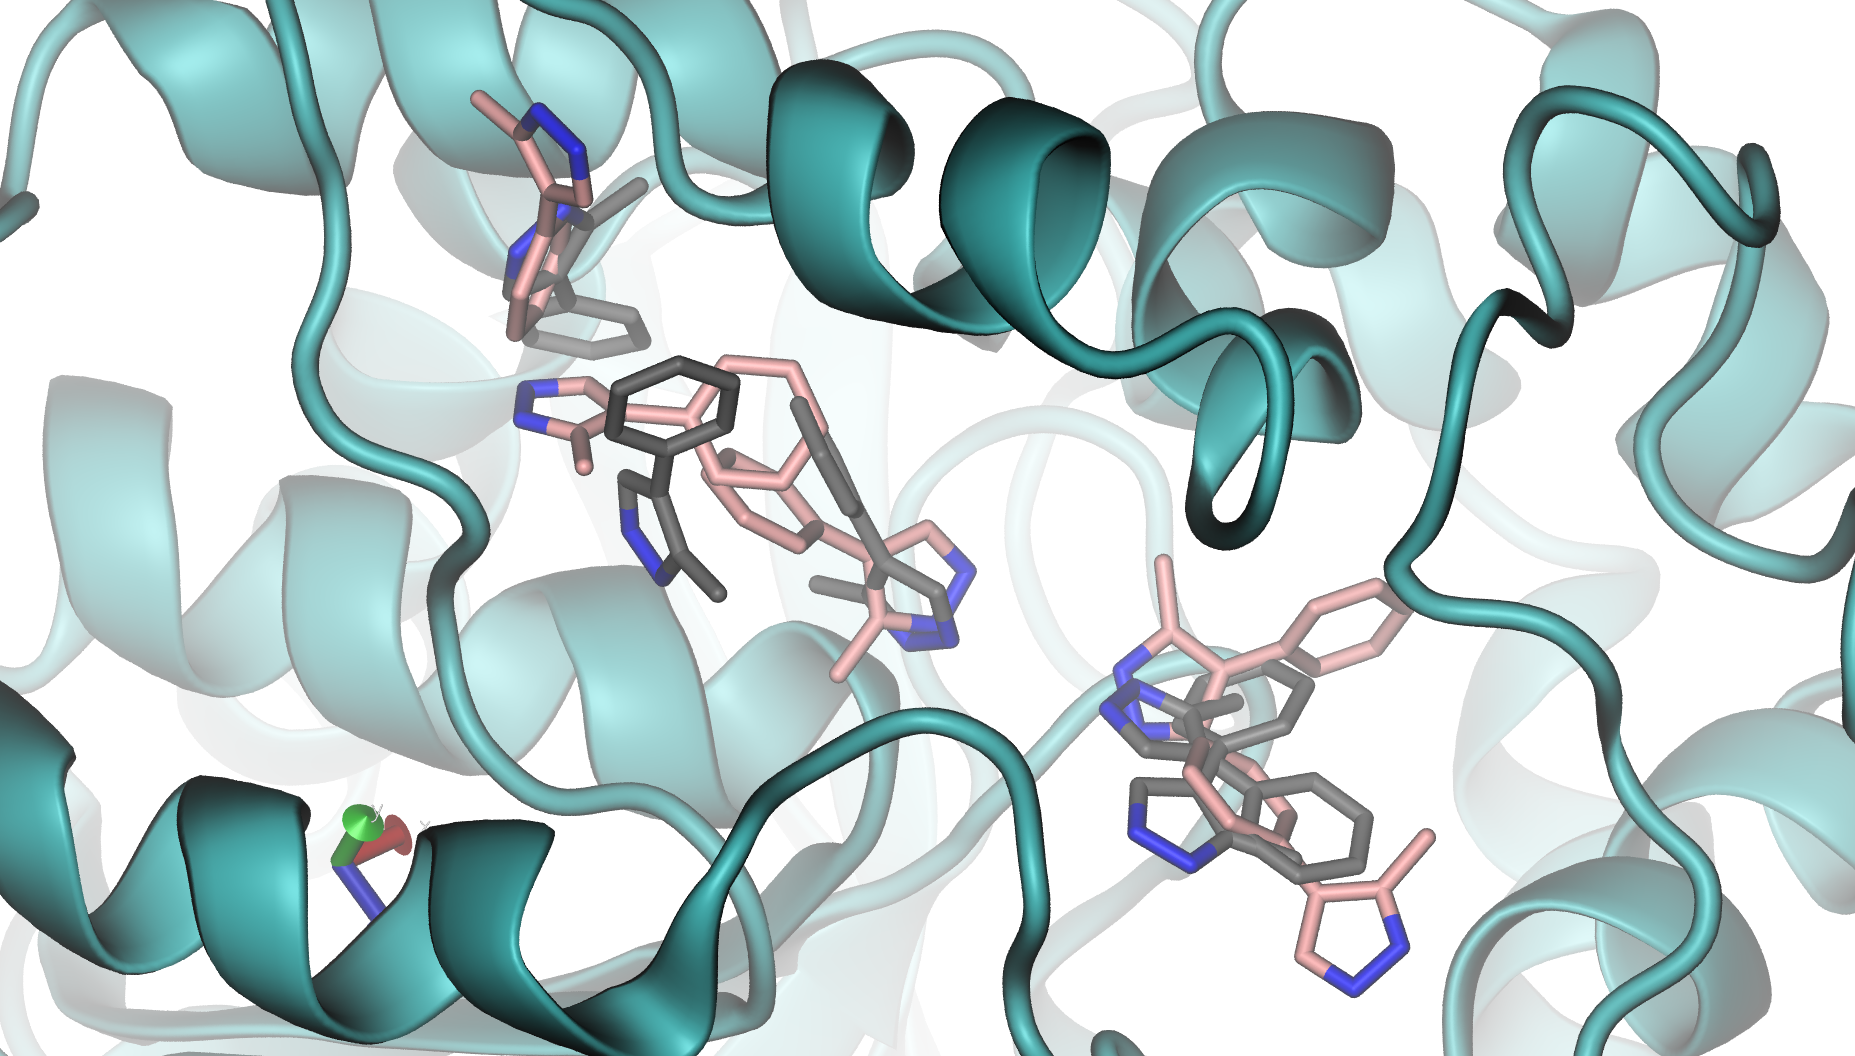
\includegraphics{chapter6/Figures/GVG_1-poses.png}
    \caption[GVG1 crystallographic binding modes]{2 crystallographic binding modes (gray/white) of GVG1 found in the right sub-cavity, overlaid with one docked pose (pink) used as our simulation starting point.}
    \label{fig:GVG1-xtal}
\end{figure}

In Figure \ref{fig:GVG1_c4-md}, we show our simulation data for GVG1 which started from one docked pose, located in the right sub-cavity (Fig. \ref{GVG1-xtal}).
In the 0-500ns timeframe, we primarily see sampling of a single binding mode (blue), but from 500-1000ns we observe several transitions between two other binding modes (red/green).
The top two most populated binding modes during our MD simulations were represented by the blue and green binding modes.
These blue and green binding modes sampled from MD were, at best (considering the minimum RMSD), 1.6{\AA} and 1.9{\AA} away from the crystallographic binding mode, respectively.
From a single 1 microsecond MD simulation, starting from one docked pose, we see sampling of 3 binding modes which enabled MD to find 2/2 crystallographic binding modes (GVG1-0,1) located in the right sub-cavity.
Since we observed sampling of additional binding modes from our simulations starting from this docked pose (c4), we would not have had to run additional MD simulations from starting from the other docked poses to identify the the secondary binding mode for GVG1.

\begin{figure}
    \centering
    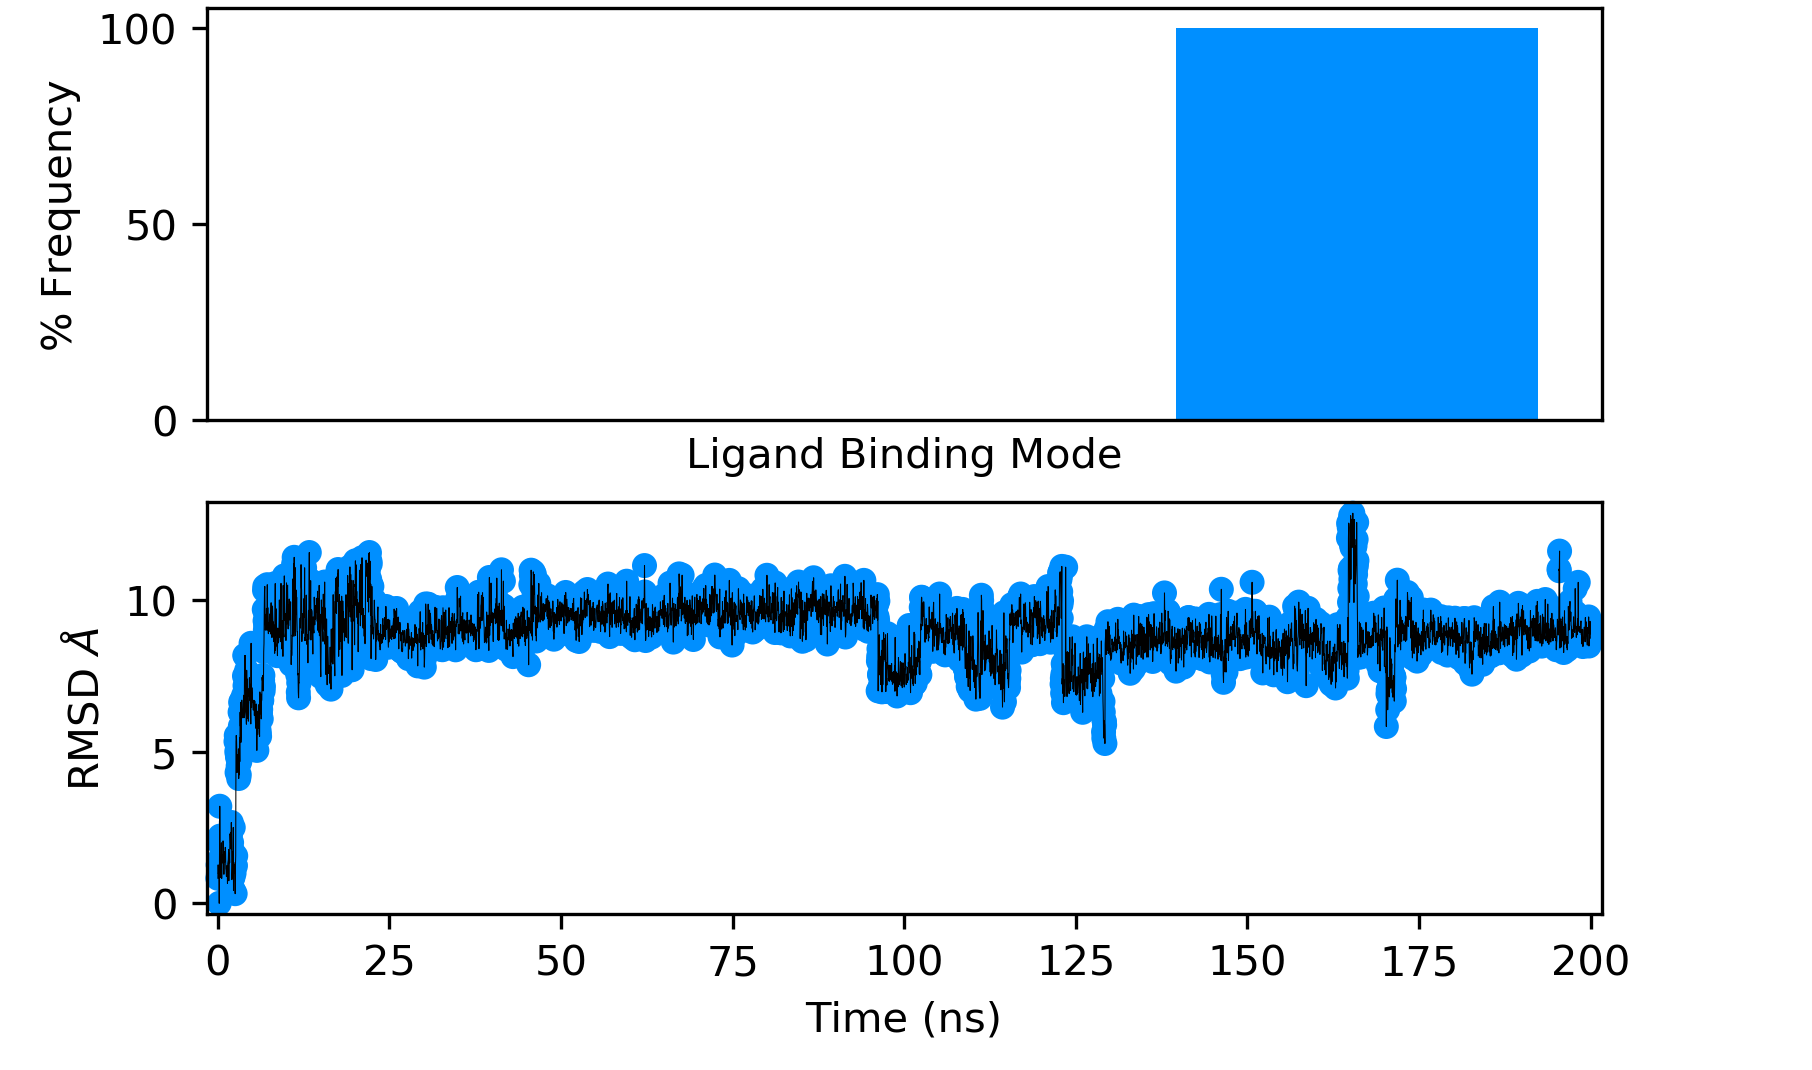
\includegraphics{chapter6/Figures/GVG_1_c4-14650607.png}
    \caption[GVG1 (c4) BLUES Populations]{Top: 200ns BLUES population (\% simulation time) of 1 (blue) binding mode sampled for ligand GVG1 starting from docked pose c4. Bottom: RMSD of ligand GVG1 relative to starting positions over time. Each time point is colored according to the binding mode the ligand is in.}
    \label{fig:GVG1_c4-blues}
\end{figure}

In contrast, we ran a total of 600ns of BLUES simulations (in 3 independent 200ns simulations) starting from the same docked pose (c4) and--surprisingly--found that within each simulation, they remained trapped in the starting configuration(Fig. \ref{fig:GVG1_c4-blues}).
That is, we only observe sampling of a single binding mode (blue) which contrasts our MD simulations which had sampled 3 binding modes.
Only by running more BLUES simulations from an alternative docked pose (Fig. \ref{fig:GVG1_c3-blues}), were we able to briefly sample a secondary binding mode (green).
The minimum RMSD of the blue binding mode to one of the crystallographic binding modes was calculated to be 1.8 {\AA} away, while the green binding mode was calculated to be 2.8 {\AA} away from the secondary binding mode found in the crystal structure.
When considering the minimum RMSD, we find that with BLUES, we are able to identify at least 1/2 crystallographic binding modes (GVG1-0), but was unable to find the secondary binding mode which we attribute to poor sampling of the green binding mode in our BLUES simulations.

\begin{figure}
    \centering
    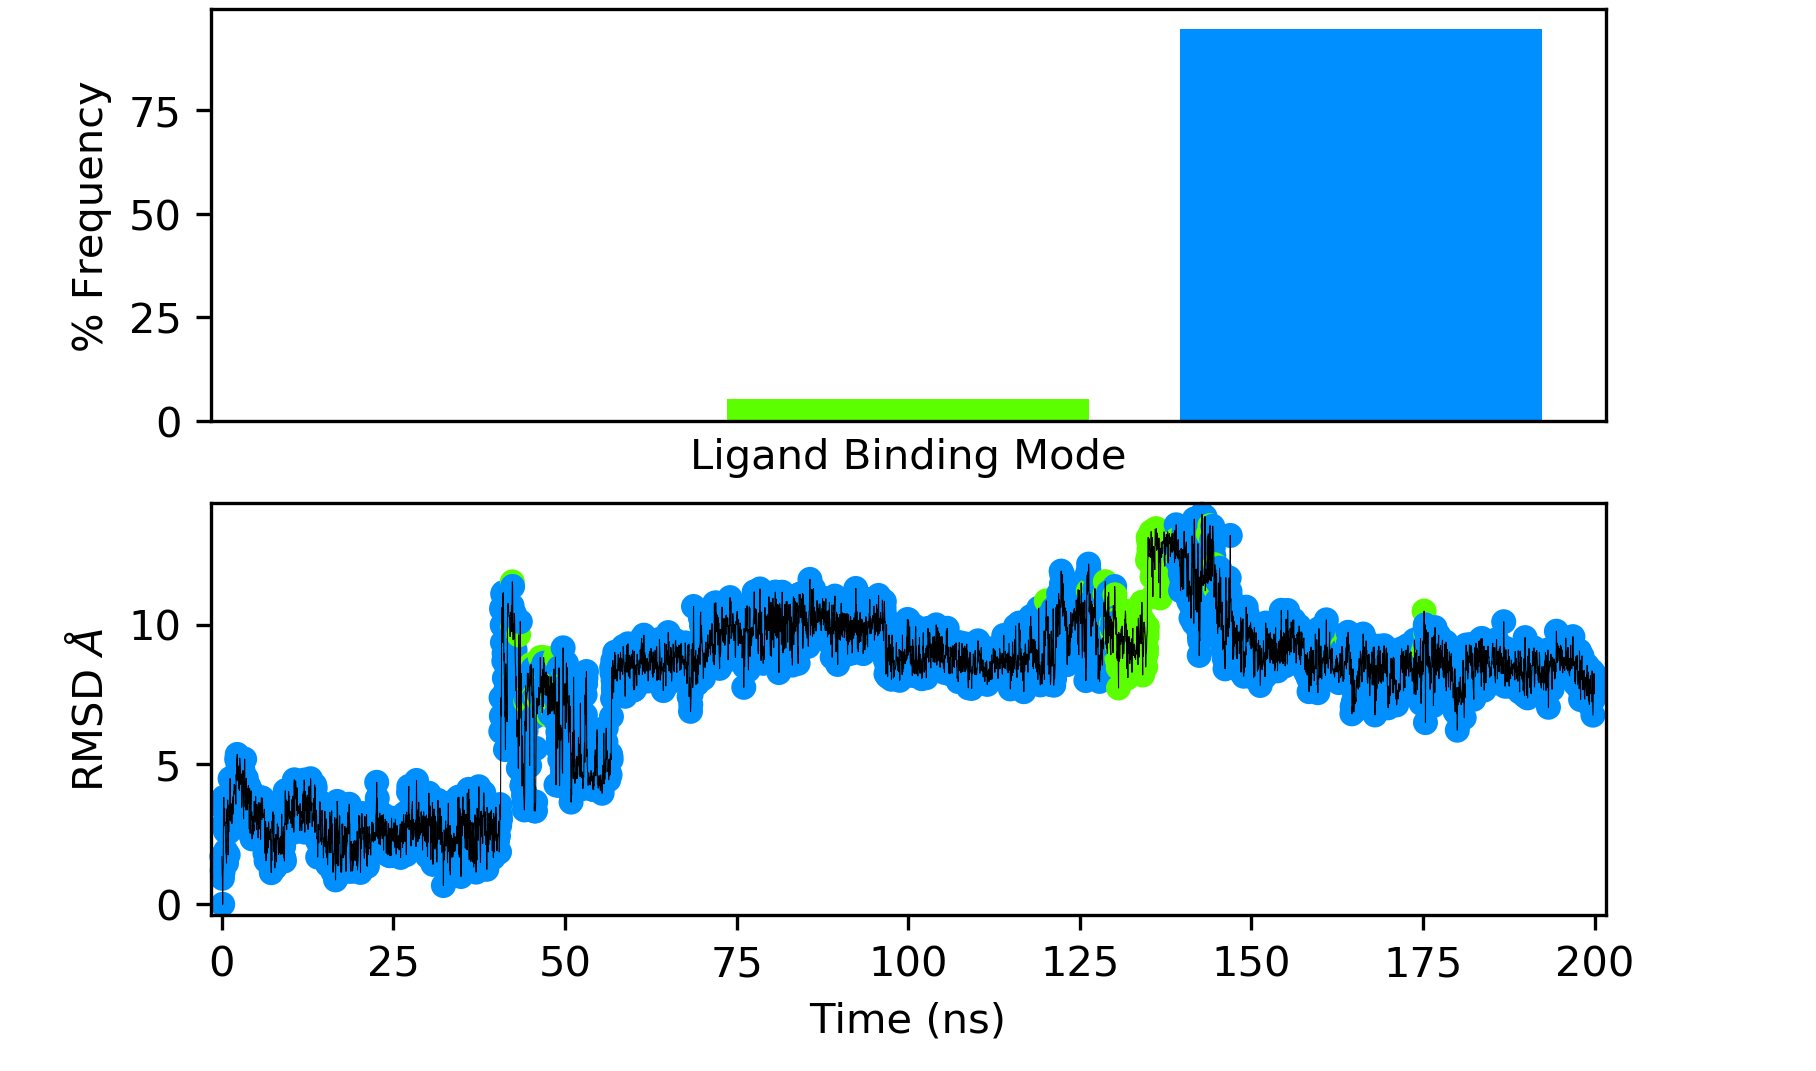
\includegraphics{chapter6/Figures/GVG_1_c3-14709106.png}
    \caption[GVG1 (c3) BLUES Populations]{Top: 200ns BLUES populations (\% simulation time) of 2 (green, blue) binding mode sampled for ligand GVG1 starting from docked pose c3. Bottom: RMSD of ligand GVG1 relative to starting positions over time. Each time point is colored according to the binding mode the ligand is in.}
    \label{fig:GVG1_c3-blues}
\end{figure}

Overall, when we consider the average RMSDs for each method, neither method will be able to make predictions which are at least close (within 4{\AA}) to the crystallographic structures, if there are multiple binding modes to identify.
If we consider the minimum RMSDs--as in having sampled near the crystallographic binding mode--docking will make close predictions with a slight improvement using MD simulations and BLUES may be able to make successful predictions (within 2 {\AA}).
Through GVG1, we saw the importance of sampling binding modes and transitions between them during the simulation as these would potentially lead to more successful or close predictions to the crystallographic structure.
This is especially important when there are multiple crystallographic binding modes to identify.
In this atypical case, we saw more transitions with MD over BLUES which lead to more success using MD in sampling near the crystallographic binding mode
For the remainder of the multiple binding mode dataset, we observed more transitions and binding mode sampling using the BLUES approach over traditional MD, which lead to more successful predictions with BLUES (Supplementary Info).
For this subset, in the best case scenario (considering the minimum RMSDs), docking had identified 2/22 (9\%) cases, MD had identified 6/22 (27\%) and BLUES had identified 9/22 (41\%).

\section{Conclusion}
In this study, we evaluated the effectiveness in identifying the crystallographic binding modes using docking, MD, and (NCMC+MD) BLUES on a set of fragment-like molecules bound to soluble-epoxide hydrolase (SEH).
We note, again, that the reported minimum RMSDs illustrates the ability to sample close to the crystallographic structure and our reported average RMSDs represents random selection of a docked pose or representative simulation frame.
When considering the minimum RMSD from docking, the closest poses would fall within 4{\AA} of the crystallographic structure and confirmed our hypothesis that the top scoring poses from docking would not be close to the crystallographic structure (Fig. \ref{fig:topscore}).

In general, we found that with our BLUES approach we sampled alternative binding modes (and transitions between them) much more, than in our microsecond MD simulations.
When considering minimum RMSD, BLUES performs much better than MD and docking (Fig. \ref{fig:averages}).
This suggests that with the BLUES approach, we sample much closer to the crystallographic structure than MD or from a docked pose.
We believe that this is due to the enhanced sampling of alternative binding modes from the random rotational moves performed during our BLUES simulations.
In very rare cases, we may observe sufficient sampling of alternative binding modes using 1 microsecond of MD, such as with GVG1; but, generally, we mainly observe the simulation remaining trapped in the starting configuration or sampling 1-2 alternative binding modes (at best).
Our findings highlight the importance of capturing binding mode transitions during simulations, which increase the chances of sampling near the true binding mode.

Overall, we showed that microsecond MD simulations of small fragment-like molecules in the large SEH binding site were unable to reasonably sample ligand binding mode transitions, even within a given sub-cavity.
While MD did do better at docking at discovering crystallographic binding modes, even with the relatively long MD simulation time, we found most simulations remained trapped in or near the binding mode they started in.
Since they often remained trapped their starting configuration, our conclusion is that the best general approach is to use a variety of starting poses from docking to get good coverage of the binding site and potentially identify the alternative binding modes.
Using BLUES, we were able to enhance the sampling of ligand binding modes over traditional MD, while even using slightly shorter simulation times (600ns of BLUES vs 1 microsecond of MD).
Ultimately, enhanced sampling via BLUES lead to an improvement in finding the crystallographic binding modes over traditional MD simulations.

\section{Contributors}
The authors would like to acknowledge the contributions from OpenEye Scientific Software: Christopher Baylyl for administering the blind challenge, Gaetano Calabro for providing us work flows for running our simulations and Gregory Warren for curating and providing us the crystal structures.

\Section{Acknowledgements}
DLM appreciates financial support from the National Institutes of Health (1R01GM108889-01 and 1R01GM124270-01A1). Financial support for N.M.L. was provided by the National Science Foundation Graduate Research Fellowship (DGE-1321846)
